\chapter{Конструирование виртуальных мультиагентных подсетей}\label{ch:ch4}

\section{Конструирование Web-ресурсов}\label{sec:ch4/sect1}

\section{Типы виртуальных сетевых агентов}\label{sec:ch4/sect2}

\subsection{Index data structure, functionality and microservices in thematic virtual museums}\label{subsec:ch4/sec2/sub1}

\subsubsection{Introduction.} Museum as nonprofit institution which responsible for preserving historical and cultural heritage, exhibit tangible and intangible to public is facing huge problem in digital era as mention in \cite{AnggaiBlekanovSergeev2014}. Museums institution are starting digitizing their collections and describe detail information in order to intensify their activities and present on the Internet as a part of public services. However, digital transformation is inevitable, museums institution must provide good impact, experiences and values to their visitors.

The thematic concept in virtual museum is one of the approaches we take in order to accelerate digital transformation of museums institution. We are combining virtual museum (VM) and information retrieval (IR) concepts in conducting information management, analytics, and focus on users-centric to enhance their experience by providing visitors’ information need within the virtual museums system.

In this research work we are preparing, investigating and conducting experiments on data access service, index construction, applying ranking algorithms and development of microservices in thematic virtual museums for speeding up disruptive innovation in museums institution.

\subsubsection{Data crawling}  In section 2 we will describe how this application data access crawling service get the content of web pages. This crawler service can take data from museums institution in text, Hypertext Markup Language (HTML), JavaScript Object Notation (JSON), or Extensible Markup Language (XML) form. We define specific web Uniform Resource Locator (URL) to crawl and run the service to obtain content pages. The crawler service maintains and run a job for specific website and not for general uses, because it ought to crawl based on characteristics of each page in those websites. As in our case we are getting the data from Registration Museum under Ministry of Education and Culture, Republic of Indonesia. There are two models web pages structure in order to get full museum collection pages as the following.

\begin{enumerate}
	\item List of collections. The crawler service directly accesses to the URL which contains list of museum collections. This URL address show 20 items per page and navigation page to identify how many pages still remain as previous or next page from the first to the end page. All URL retrieved from this page which identified as detail collection URL will be adding to download-queue.
	\item Detail of collection. This page contains detail collection information and it can be marked as end of page to be crawled. The information which contain on this page is name of museum institution, collection type, function, age, description and picture with a title.
\end{enumerate}

The crawler services automatically download the content page until all pages have been crawled. In order to prevent Internet network traffic, we are providing delay-time parameter to the crawler services, therefore this engine can be customizing to aggressive or polite crawler modes. The algorithm we are using on this task is Breadth First Search \cite{HassaanBurtscherPingali}, however the page of collection is not deep, therefore to download those pages the formula can be written as shown below:
\[
f(p) = \sum_{i = 1}^{n} \sum_{j = 1}^{m} \textit{dl }(\textit{page})
\]

\subsubsection{Parsing data} In this stage the service will parse data which has been obtained. There are two models we have been using in order to parsing data from crawler service, first we are directly parsing HTML format into Thermal VM (TVM) data schema, and second the parser service follow standard rule for data exchange. Parser service has developed for performing tasks in general, therefore data collections which obtained by crawler can be fully implemented on this service. We are using method as shown in Figure~\cref{fig:tvmMapping}.

\begin{figure}[ht]
	\centerfloat{
		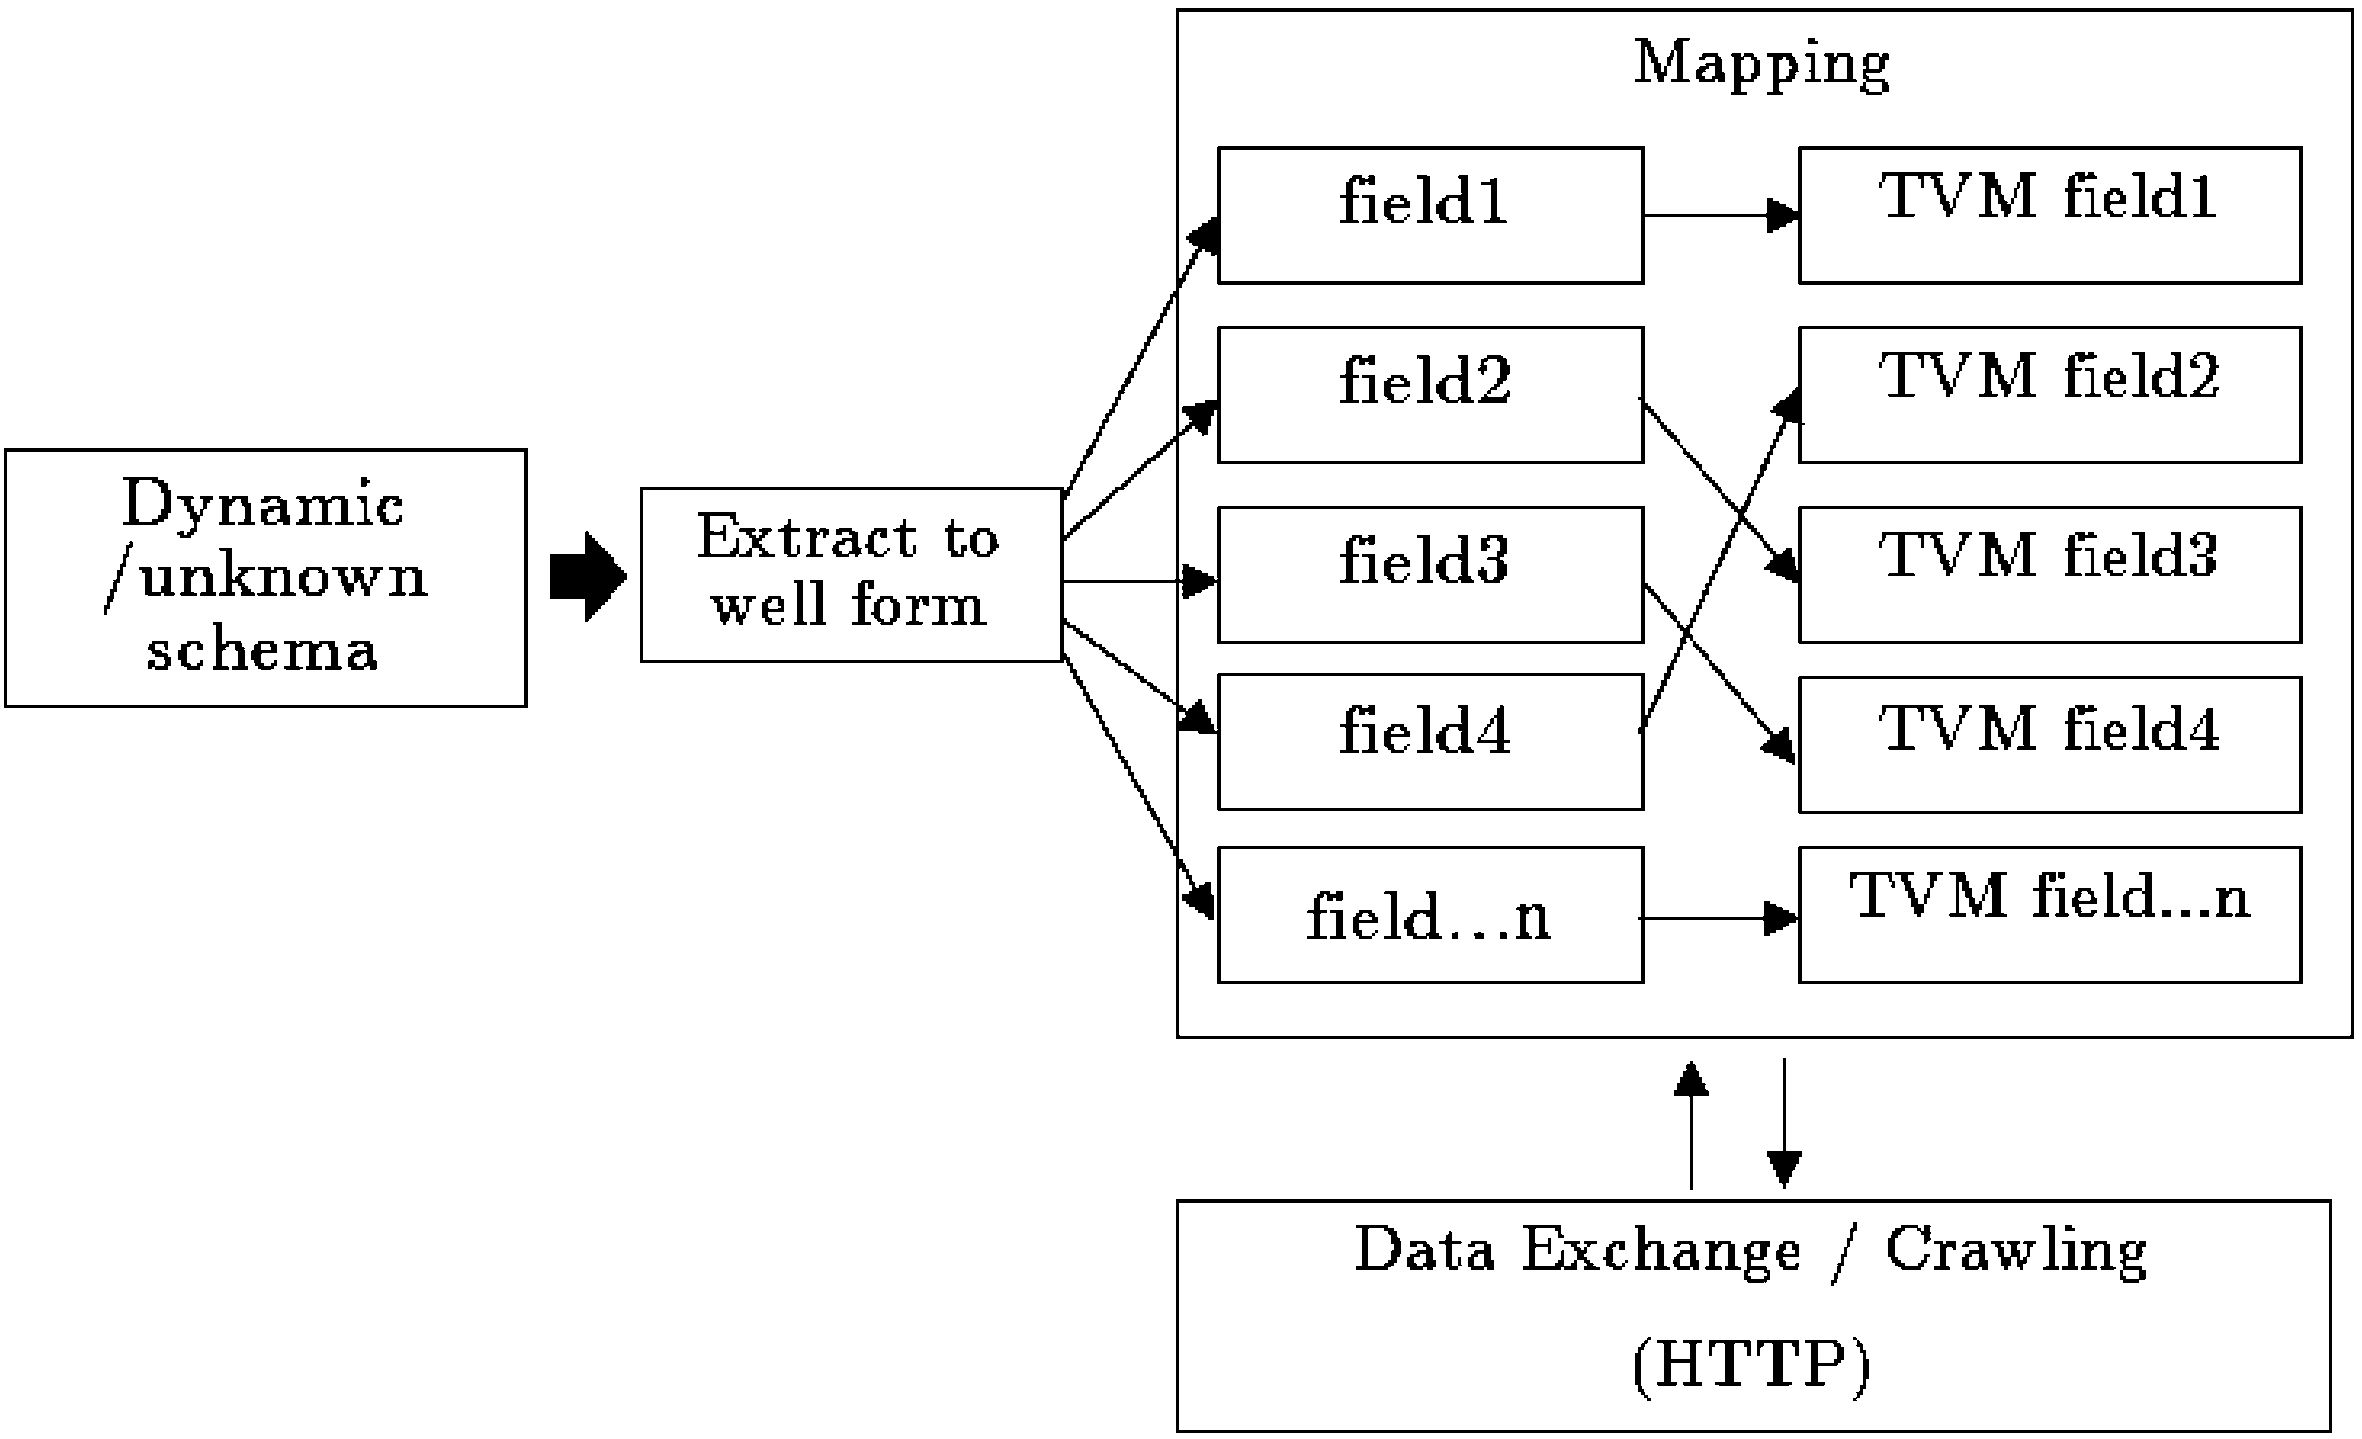
\includegraphics[scale=1]{tvmMapping}
	}
	\caption{Extracting and mapping dynamic schema to TVM schema.}\label{fig:tvmMapping}
\end{figure}

The parser service in Figure~\cref{fig:tvmMapping}, show step by step to exchange data where this service can be receiving and parsing XML or JSON format in dynamic schema includes Conceptual Interchange Documentation -- Conceptual Reference Model, Lightweight Information Describing Objects (LIDO), and Open Archives Initiative Protocol for Metadata Harvesting (OAI-PMH), however, we must define dynamic or unknown schema and extracting this schema to well form. Data exchange can be starting when the well form schema is similar with TVM schema, if not then mapping the well form schema to TVM schema should be done, only then data exchange can be performed through Hypertext Transfer Protocol (HTTP) web services.

\subsubsection{Data store} An important part of data-access service is storing and maintaining data collections which have been crawled and parsed to the standard data structure form. There are many techniques to preserve document collections, one of them is storing into databases. To store data from crawler service, we are using non-traditional database key- value MongoDB for handling structure, semi-structure and unstructured data. There are many advantages of MongoDB as mention in \cite{StanescuBrezovanBurdescu,JiaZhaoWang,WuChenJiang}, this type NoSQL document-oriented database using JSON-like format called Binary JSON (BSON), support for partition and MapReduce. MongoDB is using document store model, allow developer to create free-schema, running on multiplatform and opensource.

In our case we have developed a system to access MongoDB database server using Mgo (mango) driver for Go programming language. The Mgo driver is providing simple application programming interface, easy to use, and fast enough for performing task such as create, read, update, delete operations (\textit{https://labix.org/mgo}). The design of TVM database schema for museum collections \cite{AnggaiBlekanovSergeev2015} as shown in table~\cref{tab:tvmDbSchema} is independent and can be customized depend on the goals of spesific index task.

\begin{table} [htbp]%
	\centering
	\caption{TVM database schema for document collections.}%
	\label{tab:tvmDbSchema}% label всегда желательно идти после caption
	\renewcommand{\arraystretch}{1.6}%% Увеличение расстояния между рядами, для улучшения восприятия.
		\begin{adjustbox}{width=0.8\textwidth}
		\small
			\begin{tabulary}{\textwidth}{@{}>{\zz}L >{\zz}C >{\zz}C@{}}% Вертикальные полосы не используются принципиально, как и лишние горизонтальные (допускается по ГОСТ 2.105 пункт 4.4.5) % @{} позволяет прижиматься к краям
			\toprule     %%% верхняя линейка
			N & Key & NameDescription \\
			\midrule %%% тонкий разделитель. Отделяет названия столбцов. Обязателен по ГОСТ 2.105 пункт 4.4.5
			1 &  \_id &  Unique object identification \\ 
			2 & iddata & Identification of each data sources \\
			3 &  idinstitution &  Identification of museum institution\\ 
			4 & name & Object name or title \\ 
			5 & regcode & Registration code\\
			6 & category & Information about category or type of the object \\
			7 & collector & Person who collects the object \\ 
			8 & datefound & Date when the object was founded \\
			9 & placesfound & Places where the object was founded \\
			10 & period & Period or year of the object event happened \\
			11 & age & Age of the object \\
			12 & dimensions & Dimensions of the object\\
			13 & weight & Weight of the object \\
			14 & material & Materials forming or made of the object \\ 
			15 & condition & Description of past and recent object condition \\
			16 & totalcollection & Total object in the museum institution \\
			17 & description & Detail object description \\
			18 & ref & Reference information about where the data have been taken\\
			19 & creator & Creator of the document record in database\\
			\bottomrule %%% нижняя линейка
		\end{tabulary}%
	\end{adjustbox}
\end{table}

\subsubsection{Forward index} There are several IR techniques for document indexing system (\textit{https://www.elastic.co/blog/found-indexing-for-beginners-part3}), one of them is forward index \cite{BrinPage}, which is fast to perform task in document indexing. We are taking the museum collections data from MongoDB and managing those collections in TVM forward index. We have modified standard forward index data structure according to TVM data structure needed as shown in Figure~\cref{fig:tvmForwardIndex}.

\begin{figure}[ht]
	\centerfloat{
		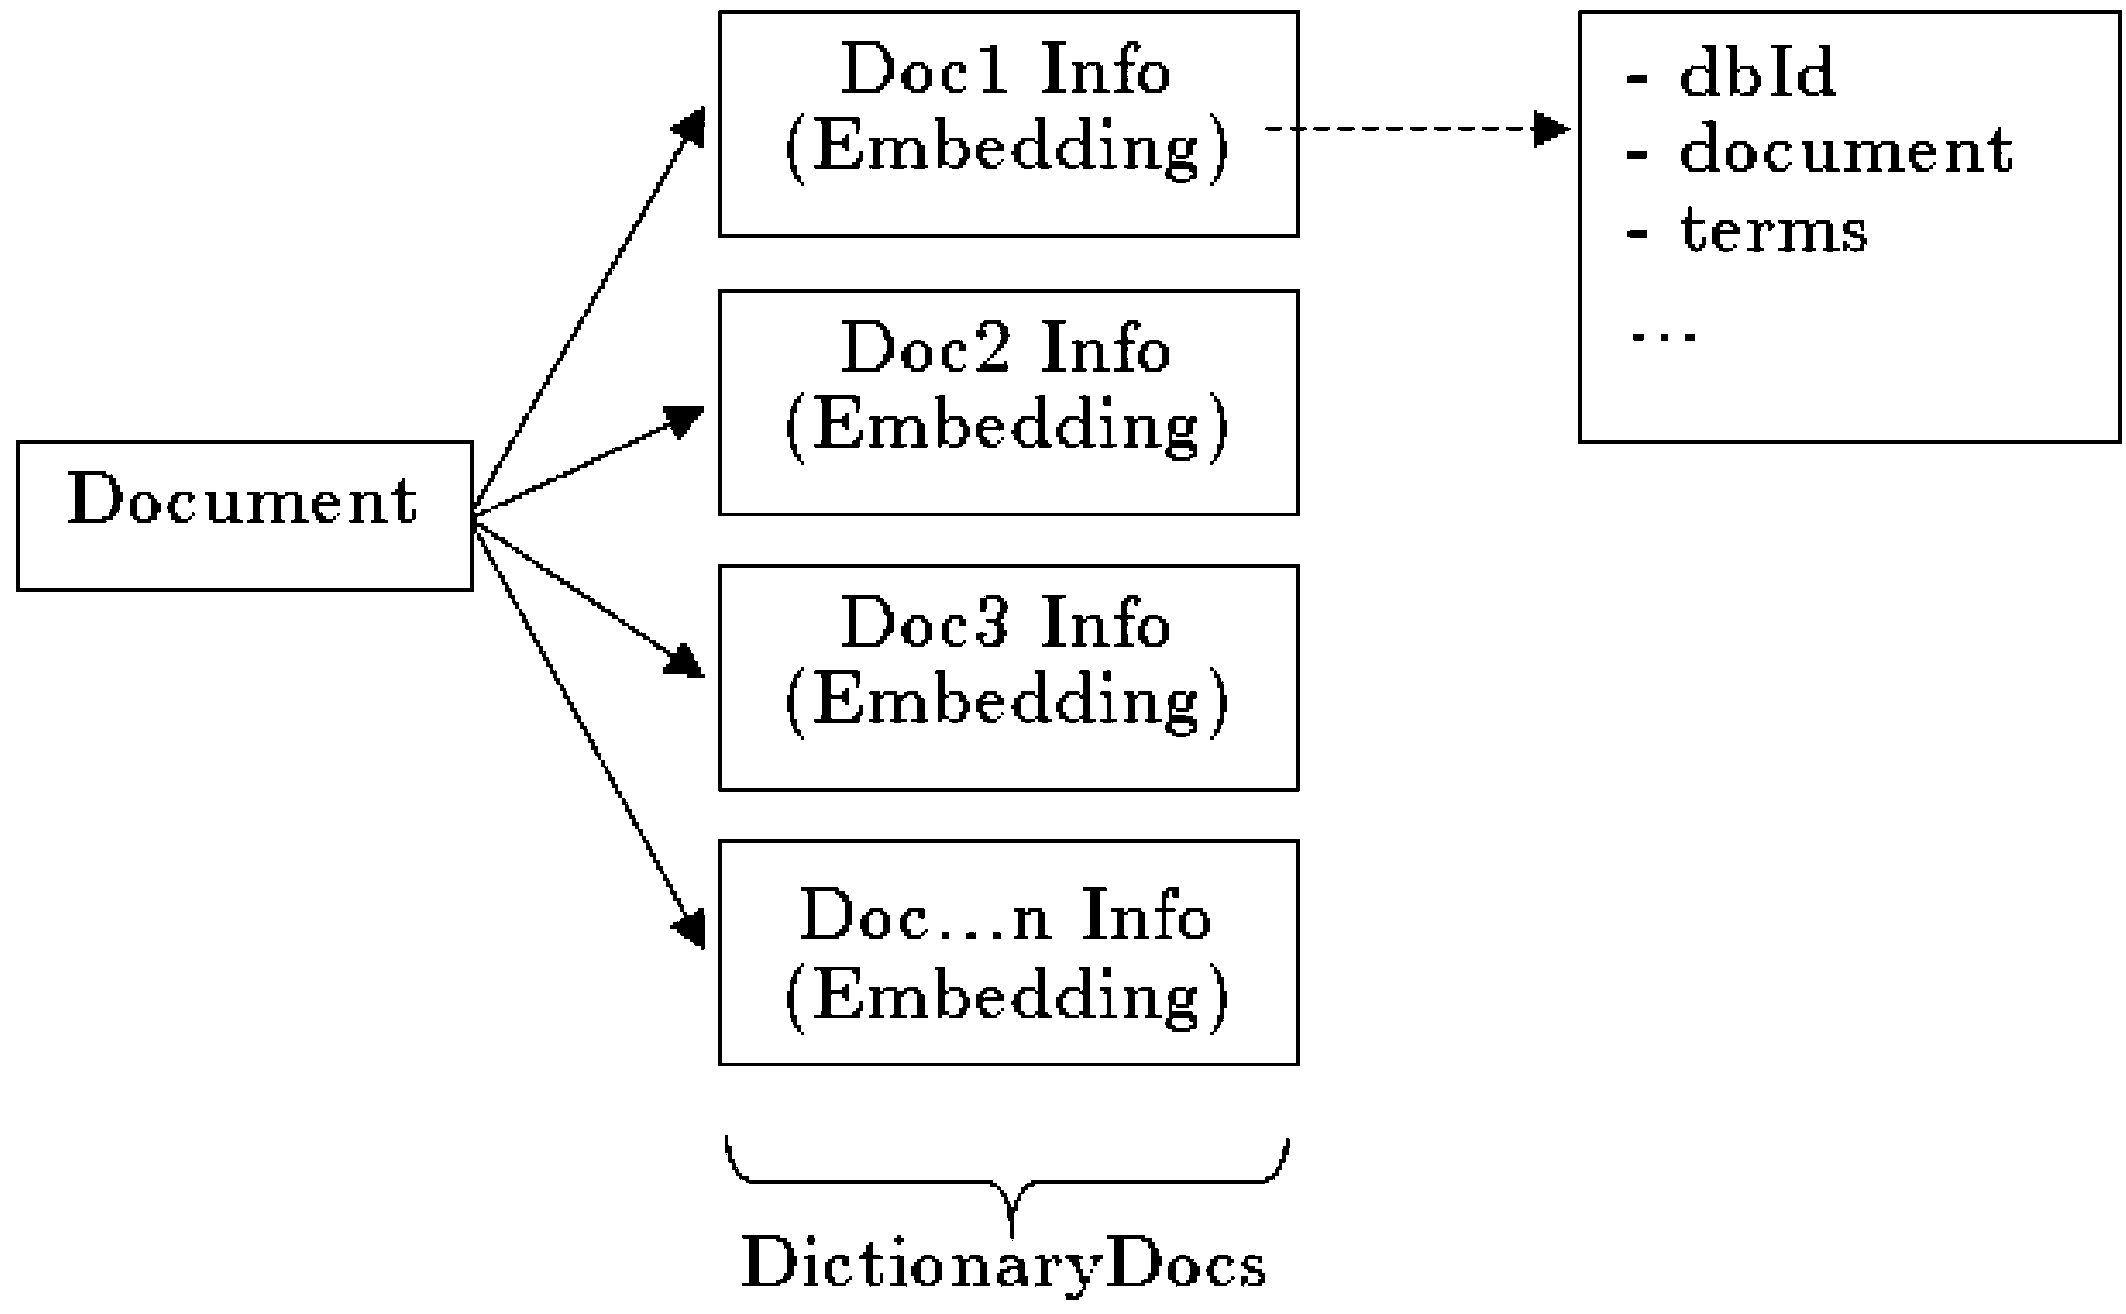
\includegraphics[scale=1]{tvmForwardIndex}
	}
	\caption{Extracting and mapping dynamic schema to TVM schema.}\label{fig:tvmForwardIndex}
\end{figure}

TVM forward index is pair document-payload using unique document identifier (DocId) for each document collections, in order to gain fast access to a document we are using hash map. Payload or embedding information in this forward index can be contains document identifier, list of terms contains in document, a record document information from database, and some necessary information. The development on flexible payload as our approach in TVM forward index give us space to embed something useful in managing and interacting with TVM inverted index.

\subsubsection{Inverted index} TVM concept which focus on fastest retrieving information need must be designed with good data structure, therefore we have created inverted index as a base for maintaining and searching information from any type application or users queries. There are many standard inverted index models have studied in \cite{ZobelMoffat,ManningRaghavanSchutze,PanevBerberich}, based on those state of the art we are modifying and designing inverted index structure for TVM need \cite{AnggaiBlekanovSergeev2017} as shown in Figure~\cref{fig:tvmInvertedIndex}.

\begin{figure}[ht]
	\centerfloat{
		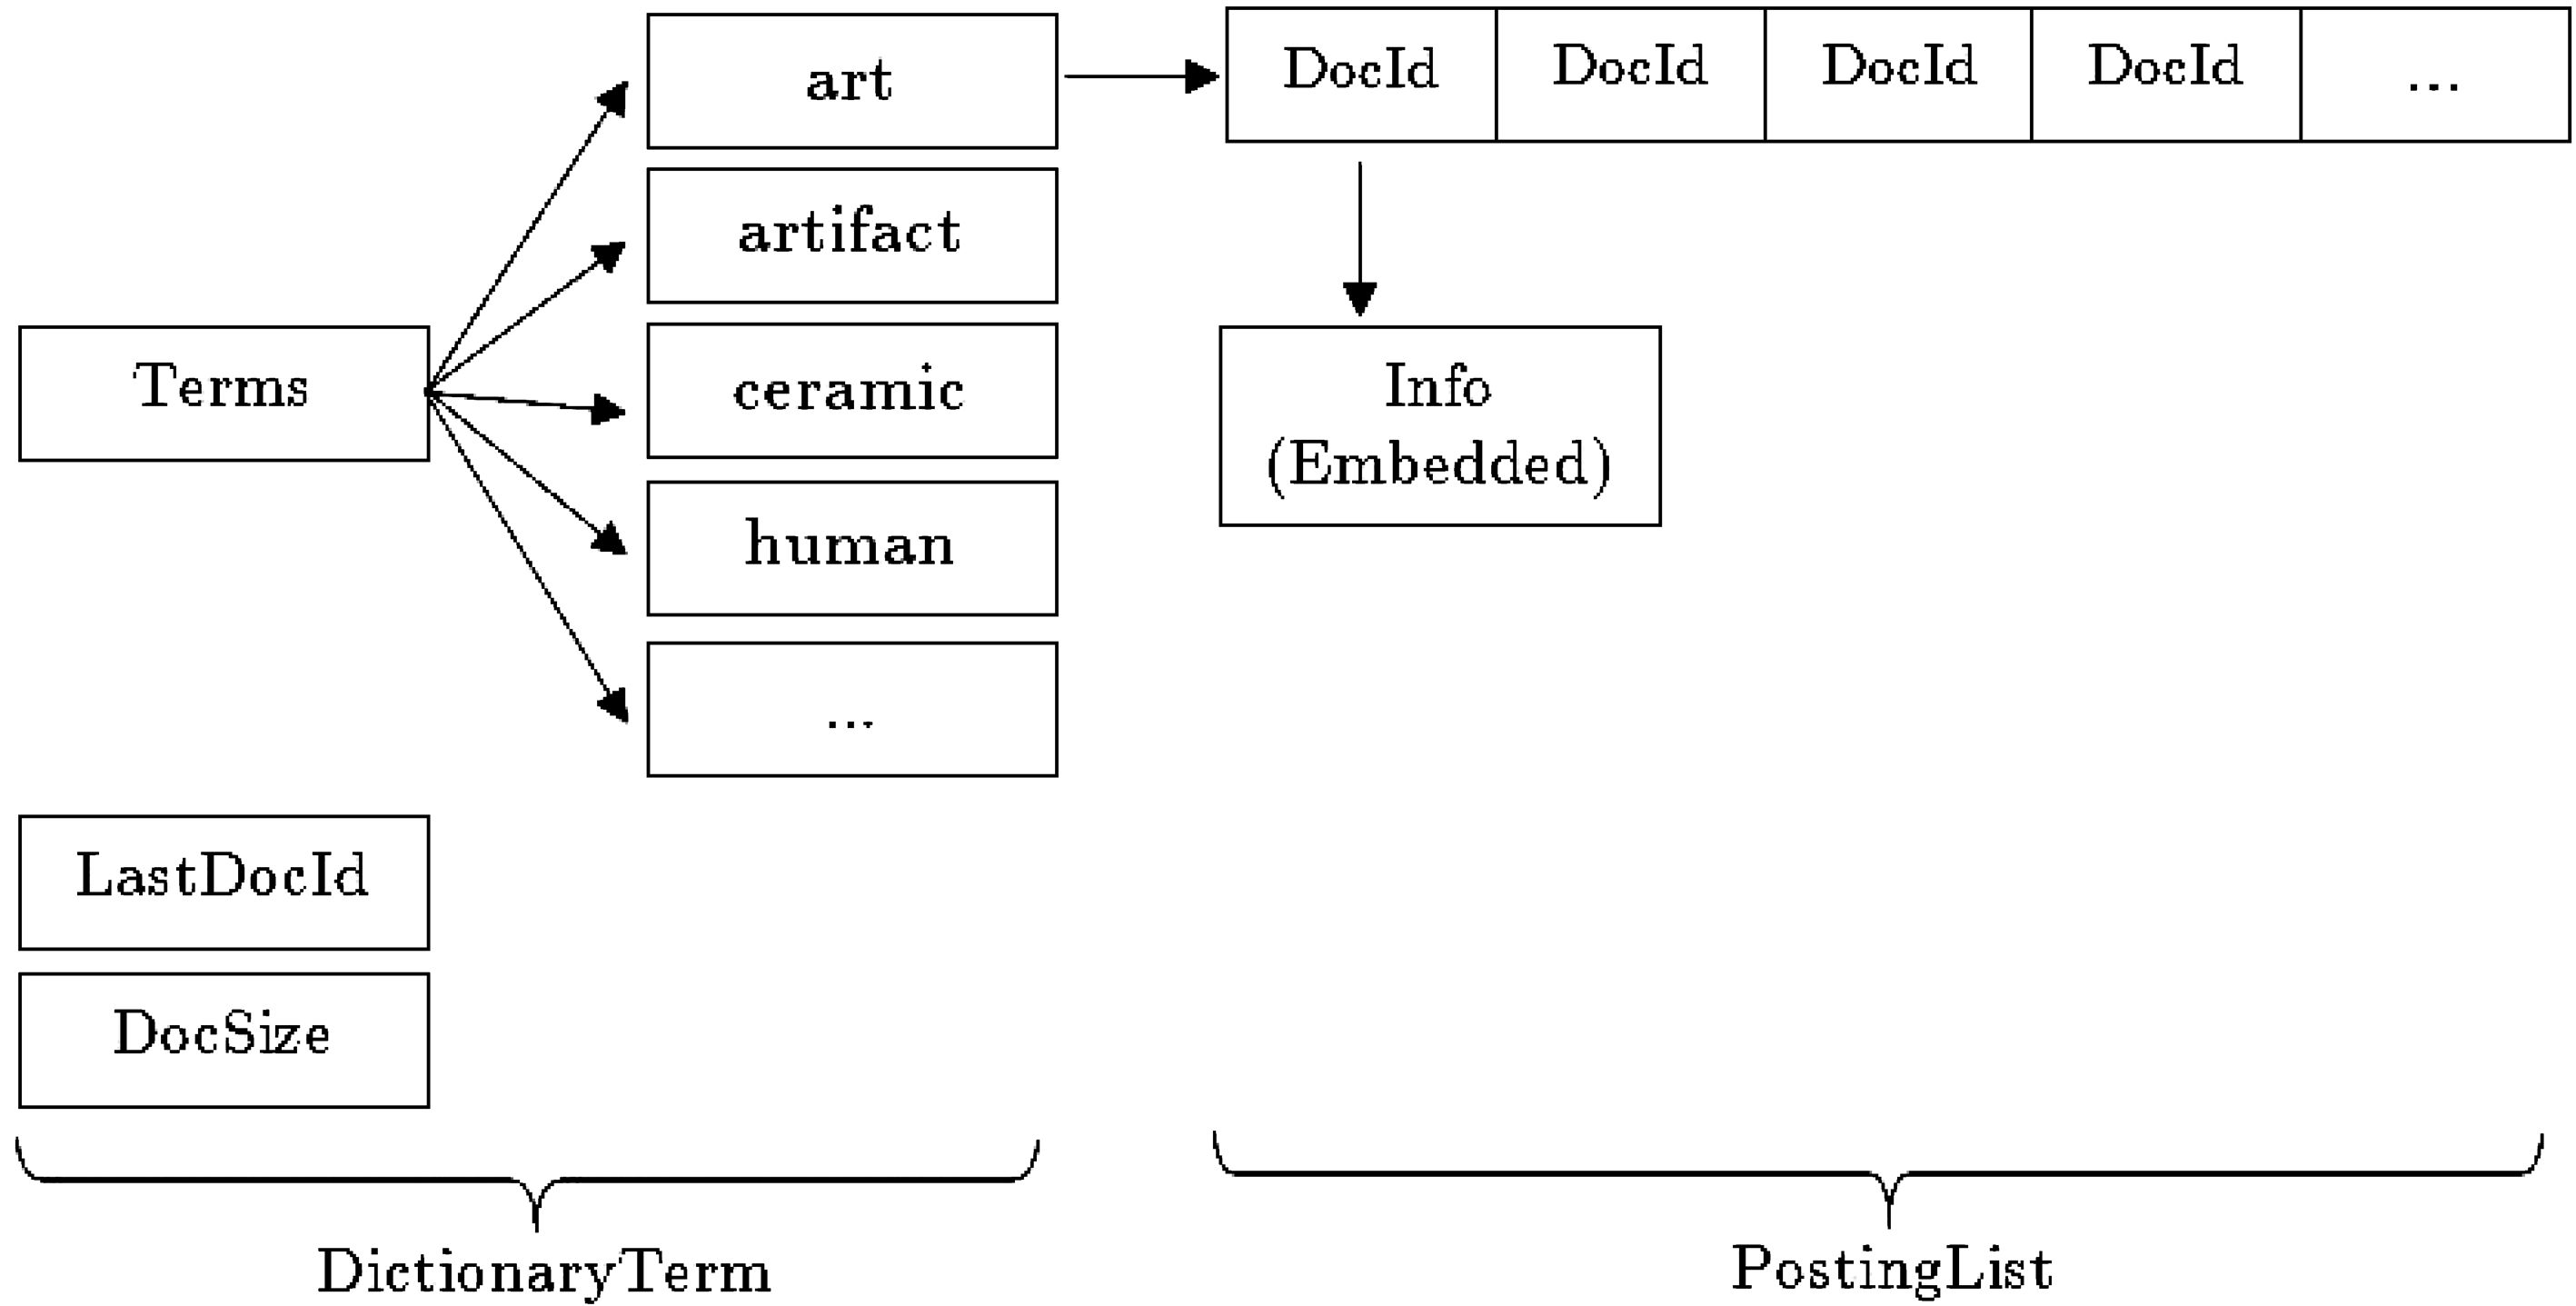
\includegraphics[scale=1]{tvmInvertedIndex}
	}
	\caption{Extracting and mapping dynamic schema to TVM schema.}\label{fig:tvmInvertedIndex}
\end{figure}

TVM inverted index maintain terms in dictionary using hash map in order to gain fast lookups, adds and deletes operations. Hash map as theoretically is performing \(O(1)\) and the worst case is \(O(n)\). Posting list for each term in dictionary also using hash map, it means that our dictionary term design is using double hash map. Access to an embedded information in this TVM inverted index will perform \(O(1)\) and the worst case is \(O(1*n)\) or \(O(n + m)\) respectively.

TVM inverted index module is providing several ranking functions such as bag of words term-frequency -- inverse document frequency (TF-IDF) \cite{ManningRaghavanSchutze}, cosine similarity measure vector space model (VSM) \cite{SaltonBuckley}, includes data provider for conceptual modeling latent semantic indexing (LSI) [9, 13] and topic modeling latent derelict allocation (LDA) \cite{BleiNgJordan}, another ranking function can be added as needed as long as it is still matching with TVM inverted index data structure design.

\subsubsection{Microservices} Index service in TVM are running on server side, therefore we have designed a microservices in order to communicate between applications, and serve requests from front-end to back-end server \cite{AnggaiBlekanovSergeev2015}. There are many benefits of microservice architecture as mentions in \cite{Singleton,GuoWangZeng,Bakshi}. TVM microservice in this case only support HTTP POST request with data submission to prevent security issue as shown in algorithm below:

\begin{figure}[ht]
	\centerfloat{
		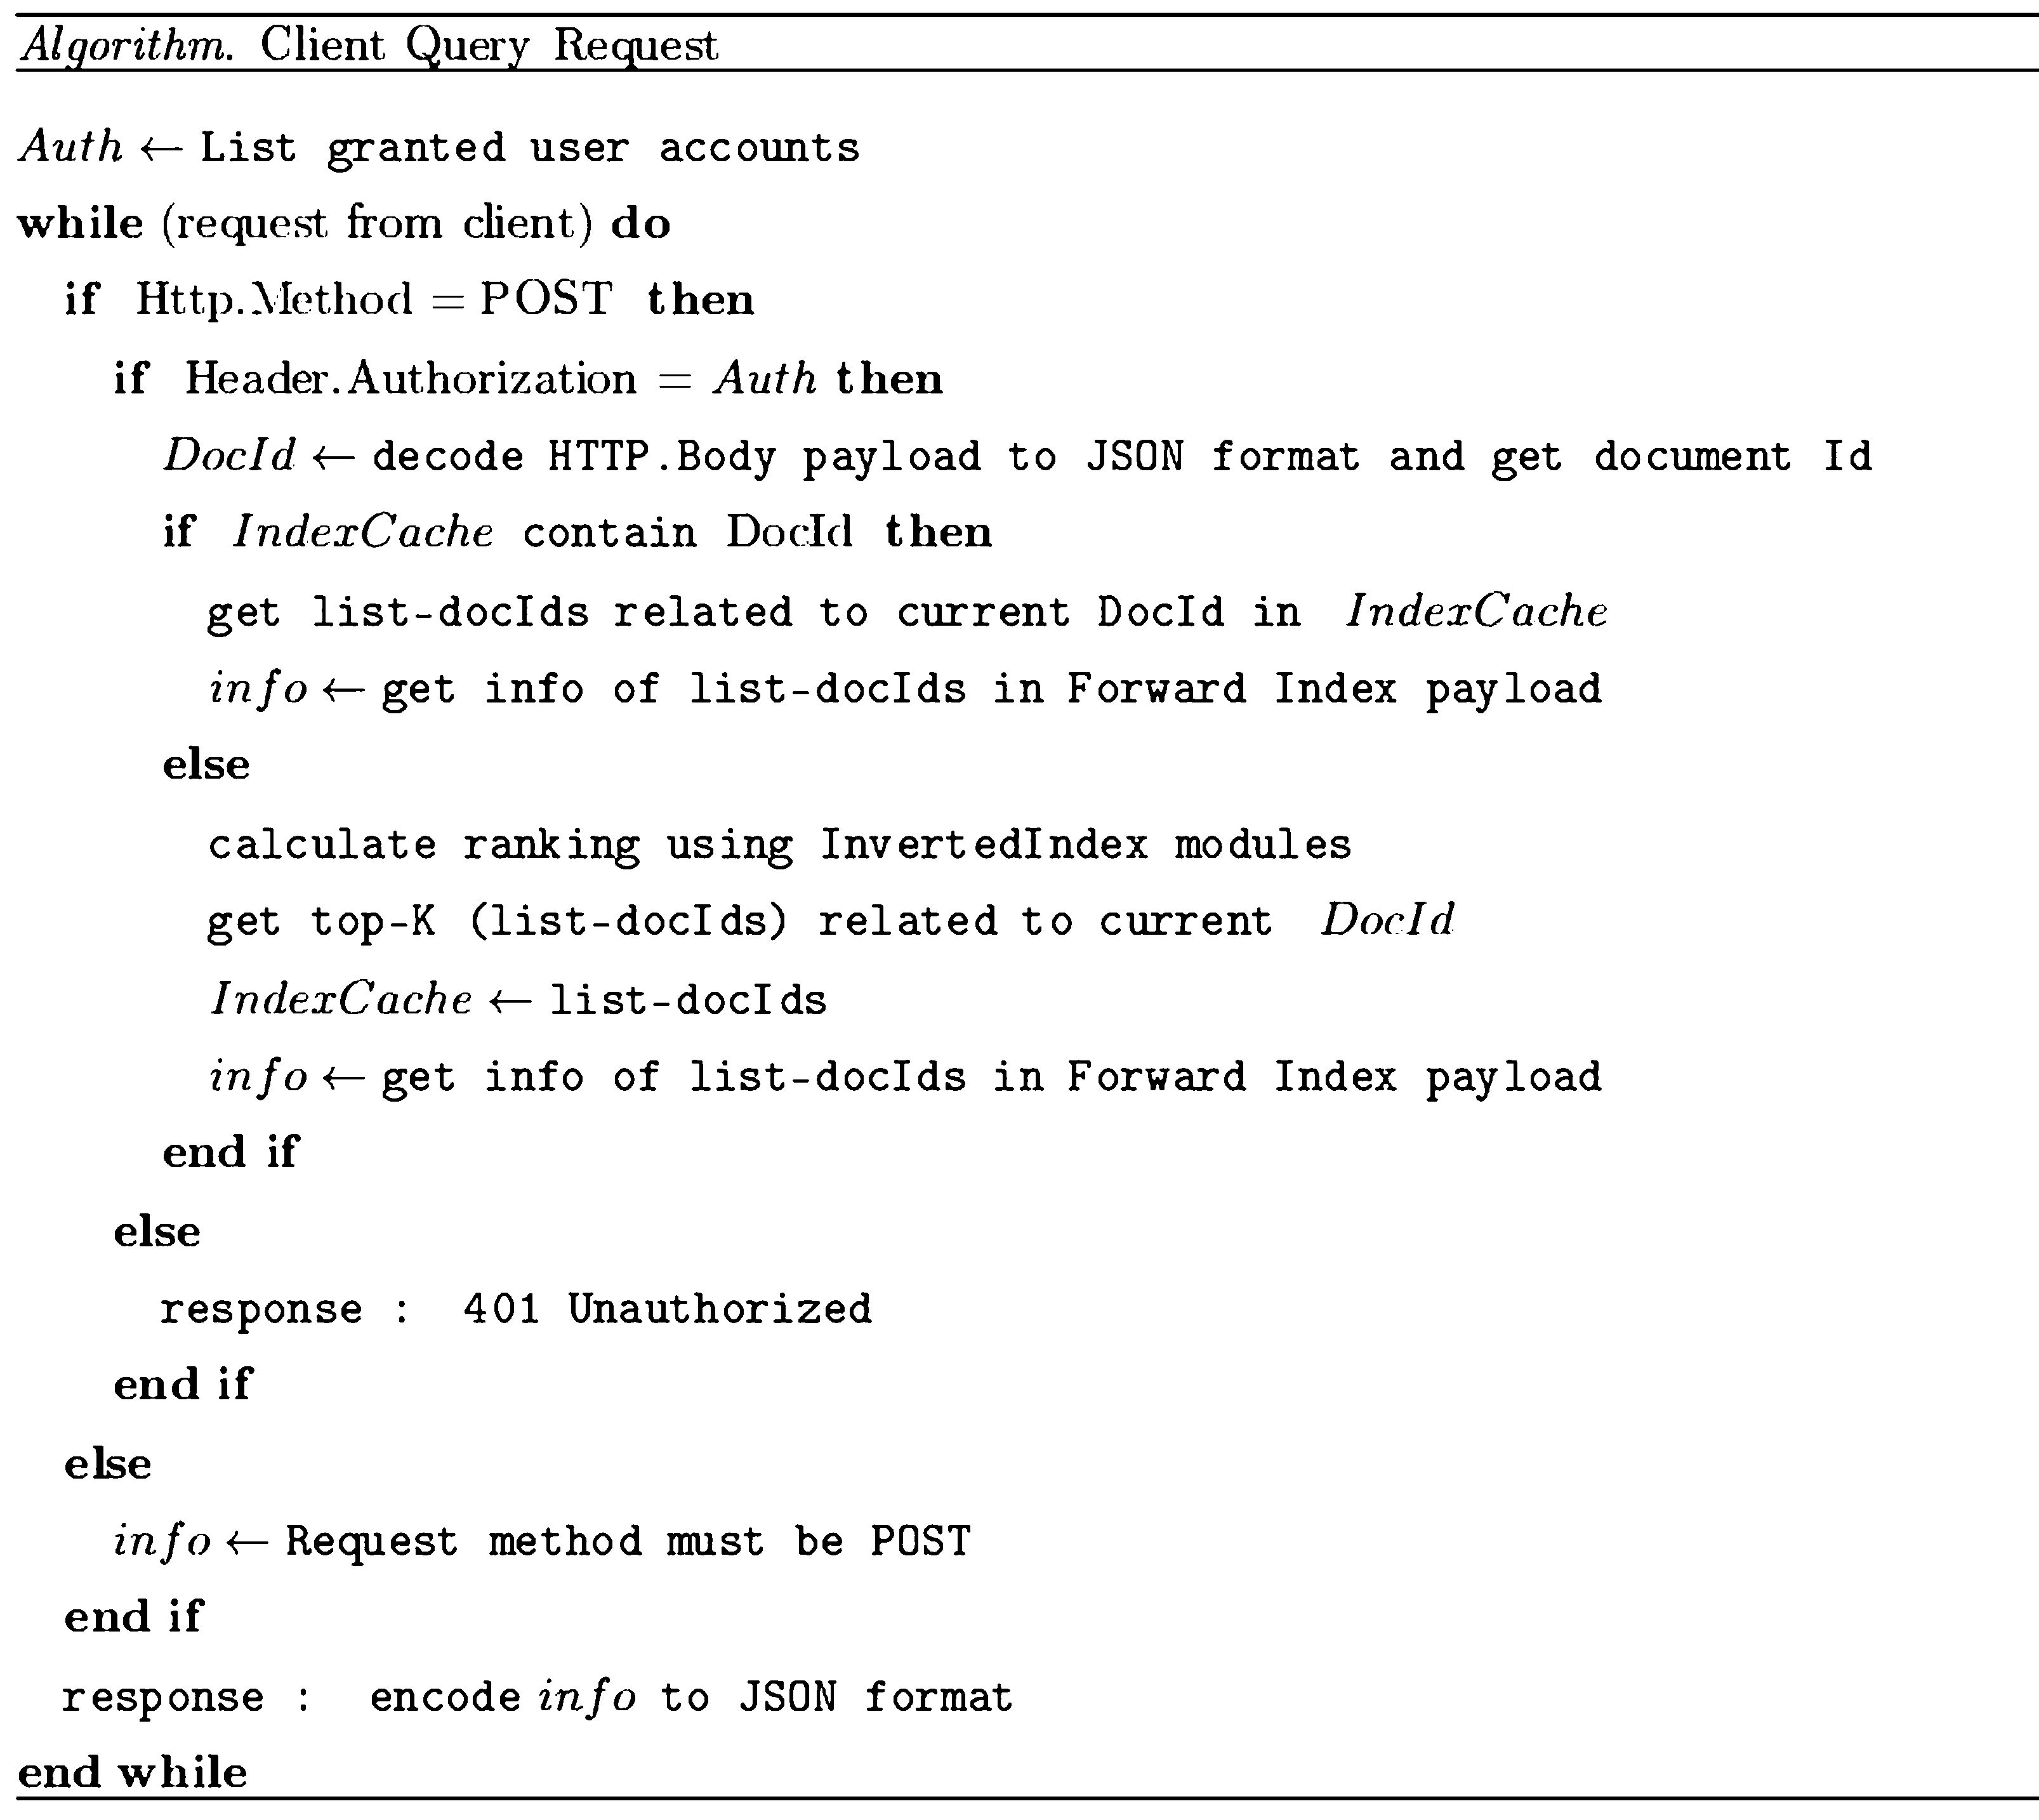
\includegraphics[scale=1]{algoQuery}
	}
	\label{fig:algoQuery}
\end{figure}

Algorithm pseudocode is describing how TVM microservice listening requests from clients, processing the request and give back a response in appropriate JSON format. HTTP header authentication schema is Basic, which transmit user and password credentials when the connection has established. The client request for searching similarity document is identified by DocId where each request will trigger inverted index ranking function and return list-docIds no more than maximum top-K ranked. The list-docId will be adding to the index-cache and using it again on the similar DocId request for reducing similar calculation process.

\subsubsection{Experiment and results} TVM system which have provided a design for microservices in this experiment will be used for handling many requests from front-end to back-end server. We have used Intel Xeon Processor 2620v4, memory DDR4 32 Gb, and hard disk Skyhawk Surveillance 2 terabyte in conducting this experiment. The data we have been using as dataset are from “Collection Museum Registration System”, Directorate Cultural Heritage Preservation and Museum, Ministry of Education and Culture, The Republic of Indonesia, which contain 29 362 collections.

In this experiment we have prepared three methods which all outputs will be encoded, written and return to the client side in JSON format, first the service will return only list of docIds form to the client in consequently allowing them to process those list of docIds for another tasks, second the service will get the list of docIds and using them as keys to identify full detail collections information in TVM forward index payload, third the service will get the list of docIds and using them to perform a query to database mongoDB for searching the detail collections information. The query request method to indicate service performance is using document at a time (DAAT) as shown in Figure~\cref{fig:daatQuery}.

\begin{figure}[ht]
	\centerfloat{
		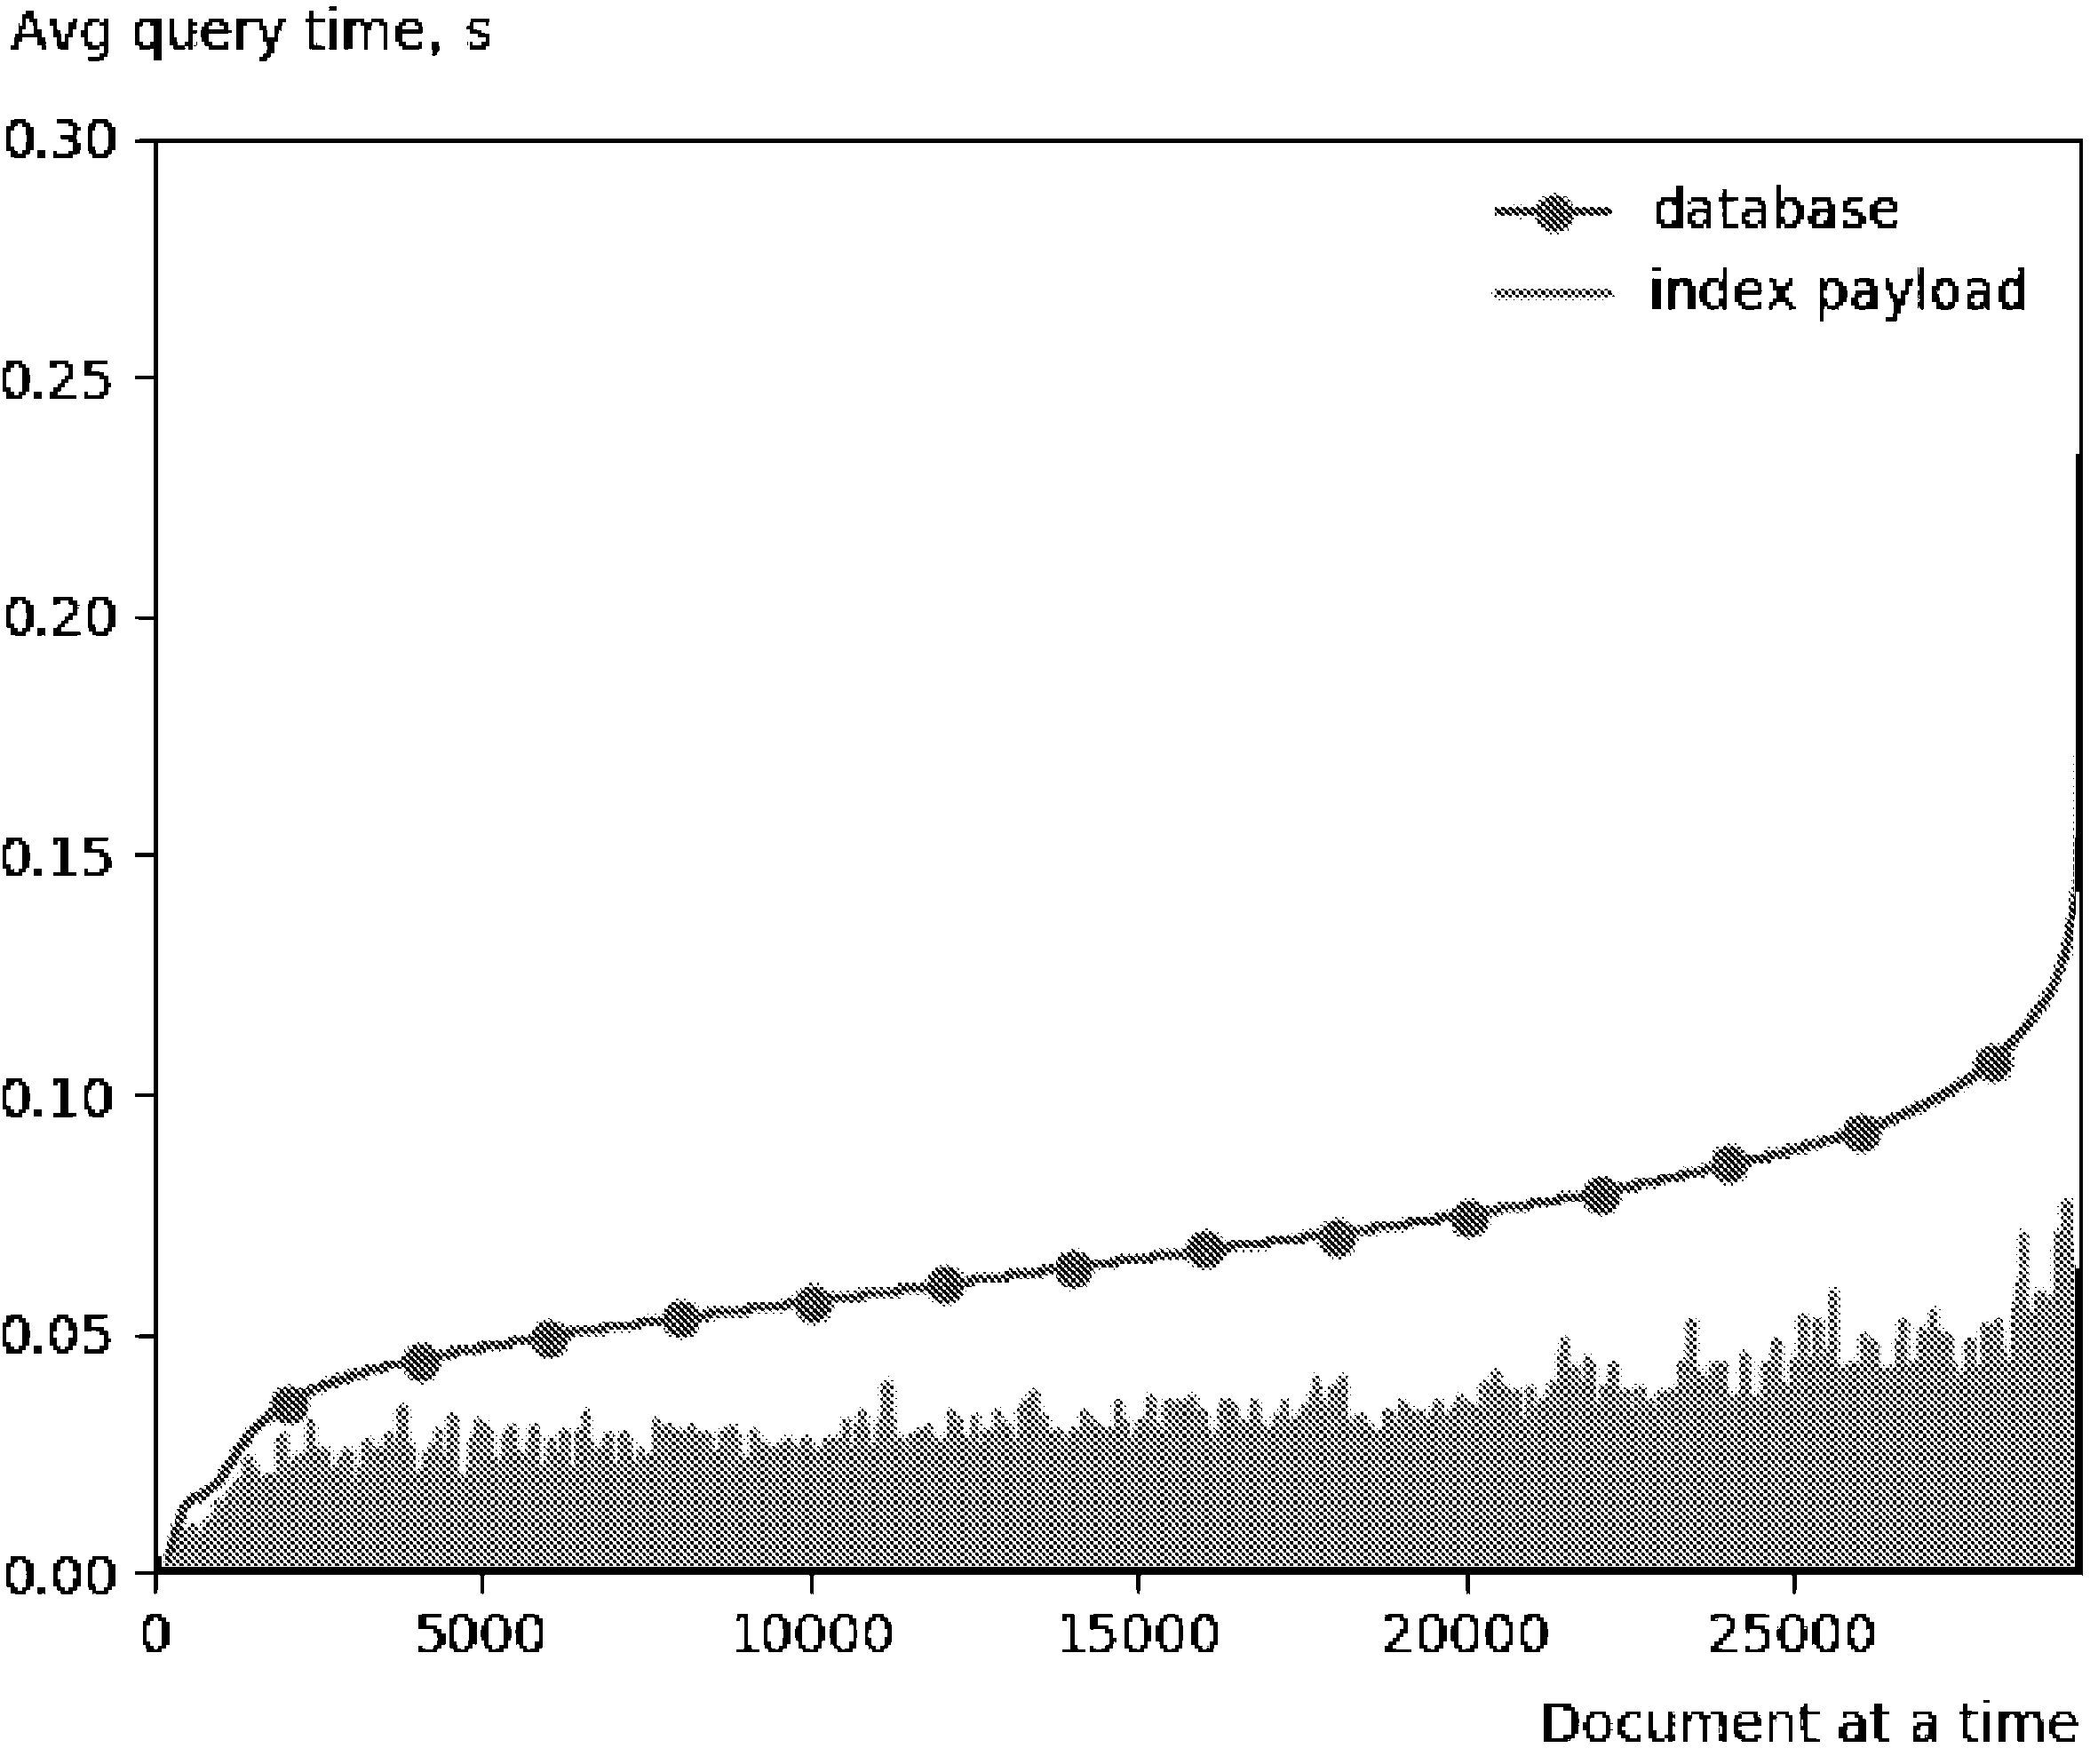
\includegraphics[scale=1]{daatQuery}
	}
	\caption{DAAT query requests from front-end to back-end server.}\label{fig:daatQuery}
\end{figure}


DAAT query request from client or front-end using appropriate JSON structure in Figure 4 was handled by TVM independent microservices where after query has performed, then inverted index function directly calculates documents score and the function returned list of top-K ranking in list of docIds form. The query processing time for accessing information to database is 84.5\% and access to index payload only need 0.02\% from total query request time.

The second experiment, we are using query term at a time (TAAT), where each term in TVM inverted index dictionary have been using for query requests in order to evaluate and calculating documents score which have contained in postings list. The result as shown in Figure~\cref{fig:taatQuery} is describing query time to database need 99.4\% and query to TVM index payload only 0.0005\% from total query request time.

\begin{figure}[ht]
	\centerfloat{
		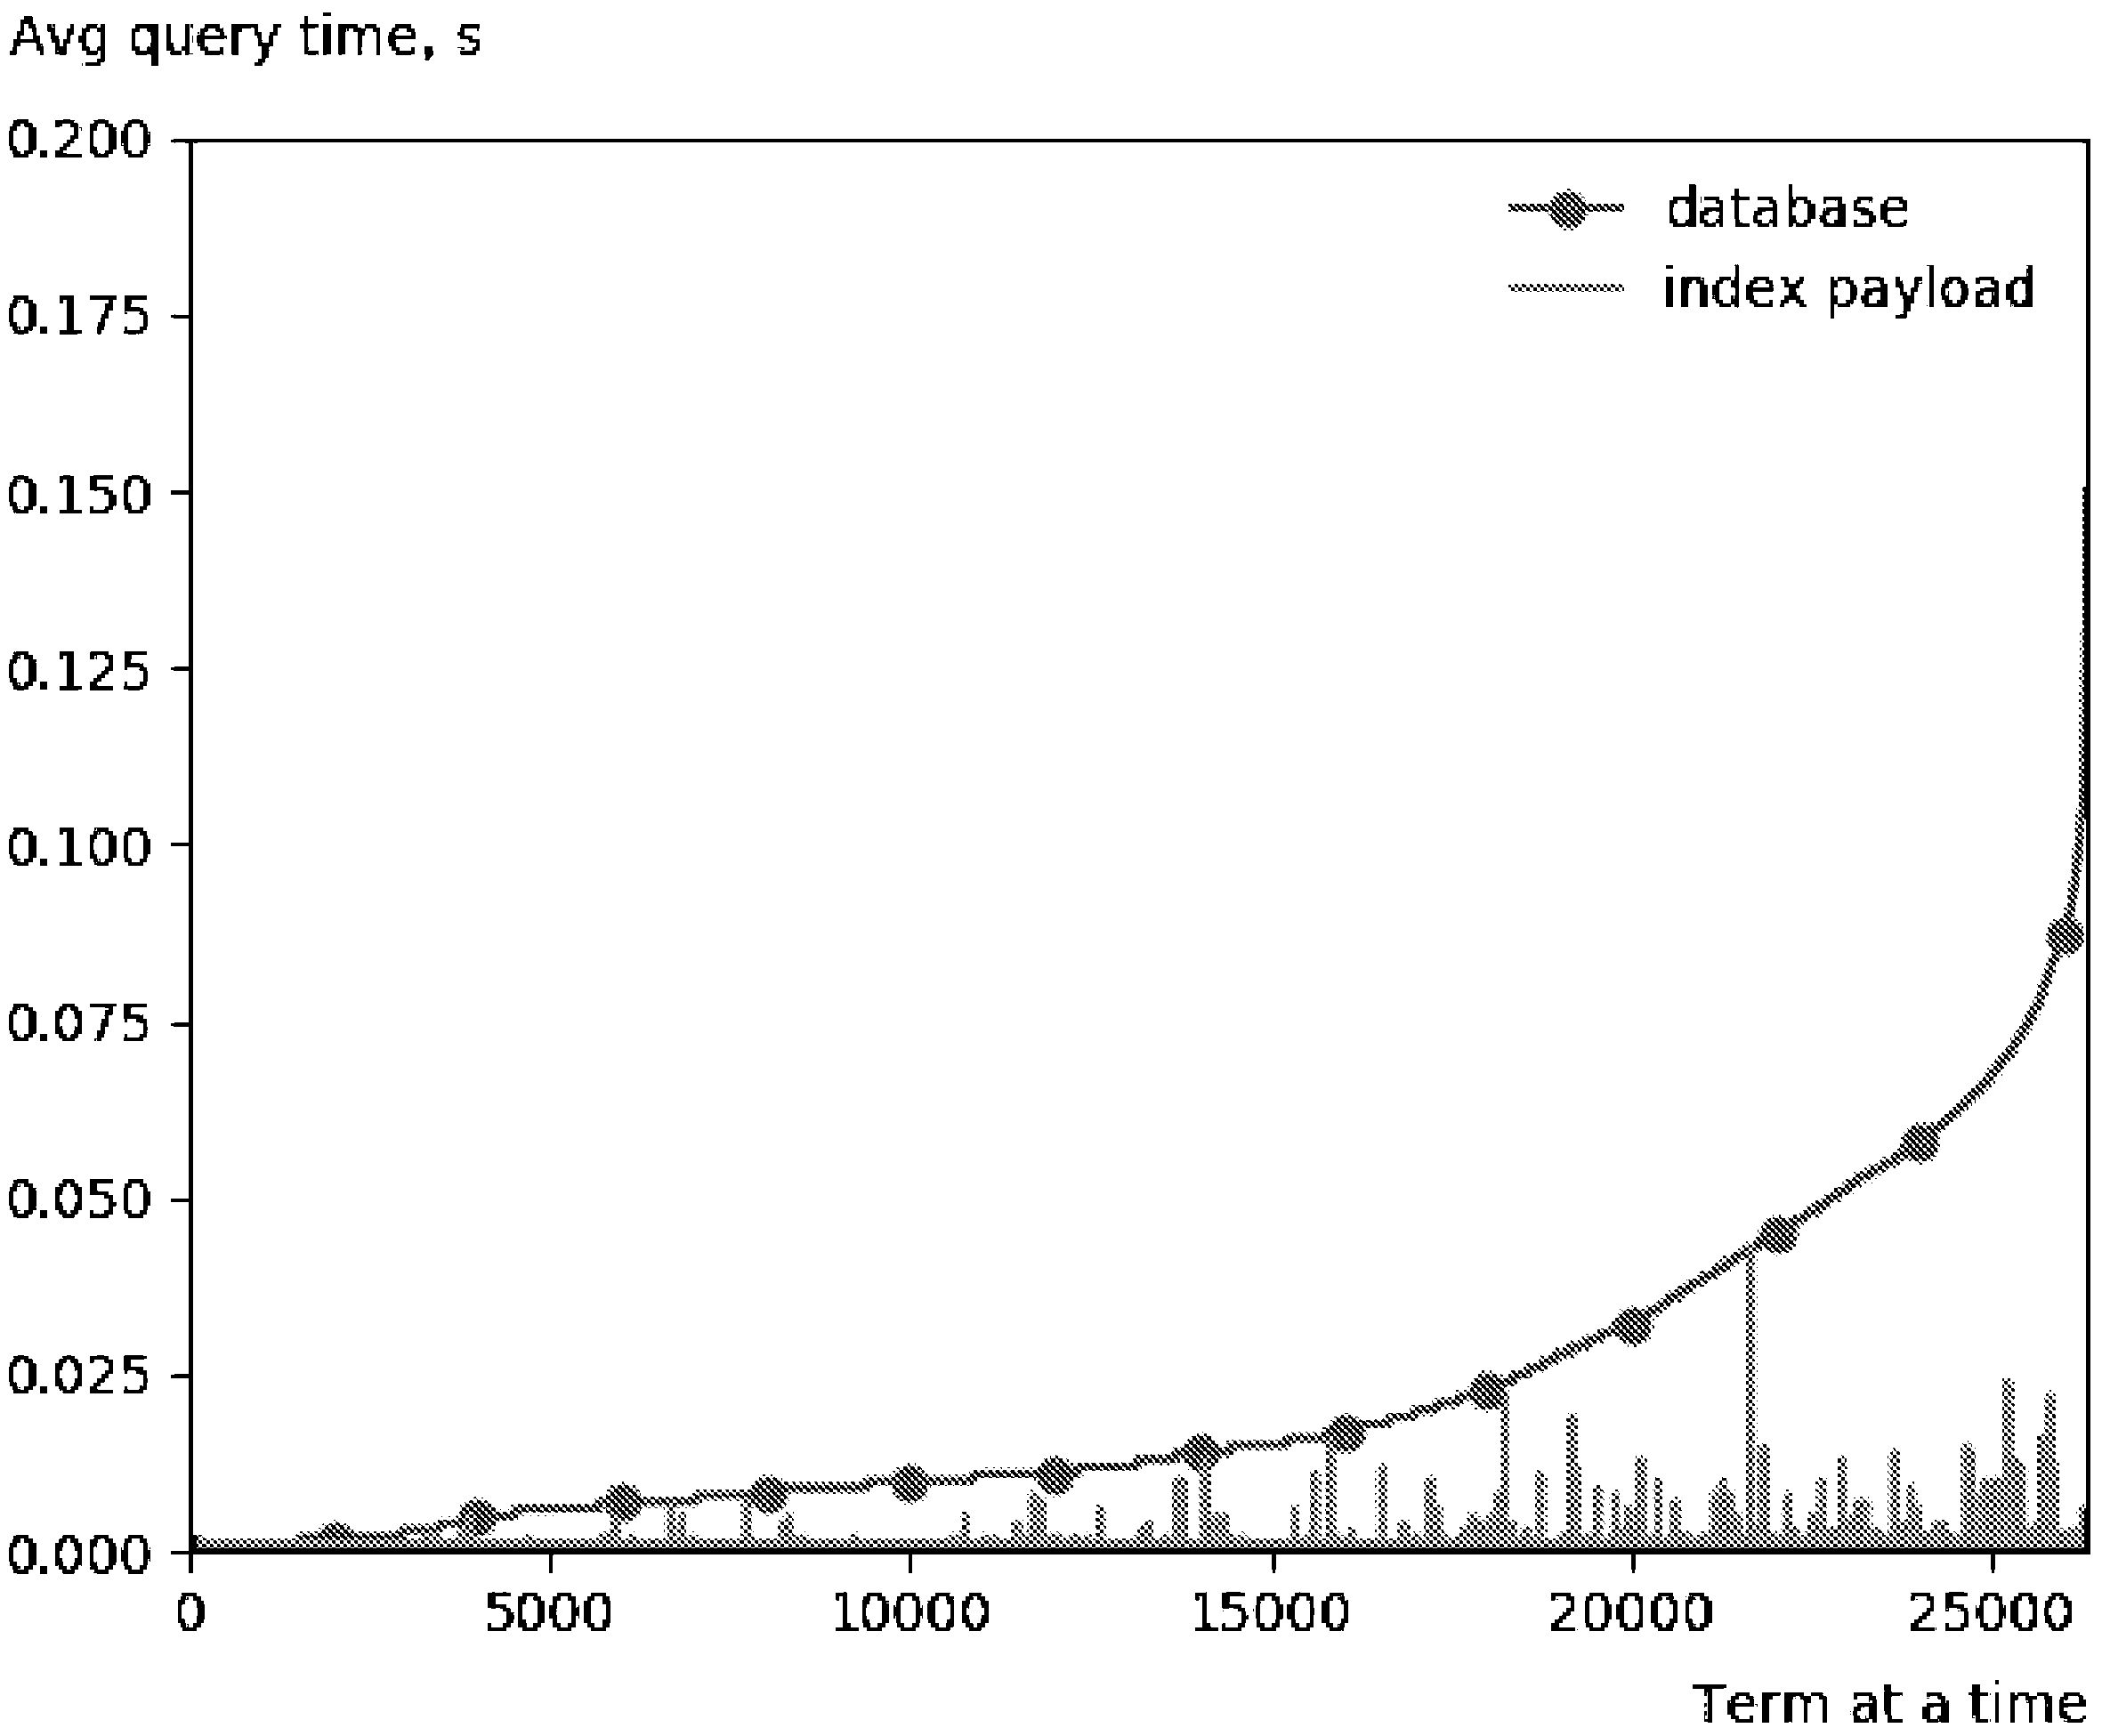
\includegraphics[scale=1]{taatQuery}
	}
	\caption{TAAT query requests from front-end to back-end server.}\label{fig:taatQuery}
\end{figure}

The first method is only gives docIds list rather than give a full information, therefore there is no request needed to database or index payload, beside this docIds list can be used as caching for top-K docIds ranking in order to reduce computation time in back-end server. The cache key is docId of recent document which is using as query request, and the value is containing array set of documents identification. The second and third methods give us a significant result, where our method have provided an access to collaborate between TVM inverted index and forward index by given embedded information as payload. Our experiments shown that the methods have been proposed can reduced time to access a detail information of the collection rather than given many direct queries to database system.

\subsubsection{Conclusion} In this work we have constructed data access service, modified forward and inverted index, and design special microservice architecture for TVM to provide relevant information for the virtual museums visitors. There are several experiments we have conducted, and shown our methodology give significant results when exchanged an information and collaborated between TVM forward and inverted index, query request, process and response through microservices give high performance output. Dynamic or flexible payload in TVM indices structure can be used for multipurpose indexing method in the development of modern information retrieval.

\subsection{Construction inverted index for dynamic collections visualization in thematic virtual museums system}\label{subsec:ch4/sec2/sub2}

\subsubsection{Introduction}

hematic virtual museum system main goal is providing more relevant information based on user characteristic, behavior and desire. Thematic exhibition as main unique feature is very considering on users’ whole activities. Thematic concept can increase user experience, deep knowledge, discovery new related content, explore unexplored, and most important thing is not disturb users by providing irrelevant information.

Barry and Maria define the creation of new knowledge, transformative and self-directed experiences, engagement with the full diversity of visitors, and transparency as the source of a viewpoint of the exhibition as museum specific evaluation criteria. Museum exhibition is not a book on the wall rather than leading visitors to new attitudes, values and ideas even in very different cultural backgrounds or religious beliefs \cite{LordPiacente}.

Interpretation of tangible and intangible cultural and natural heritage can be spread in various recent devices of information and communication technology to the end-users. The system initiative to serve users by providing accurate museum collections information which can be delivered through desktop, web or mobile application in real time. The system can help curator or museum administrator for research, clarify, grouping, visualizing and design thematic event exhibition in some cases.

John H Falk writes that most museum visitors mentioned that visitor go to museums in their free time in order to have fun and enjoy themselves or to see new interesting things in a relaxing and aesthetically pleasing setting \cite{Falk}.

The system with interactive information in the thematic exhibition which has been processing and delivering to the user will be leading to the better understanding by traveling in similar fields i.e. art, archeology, artefact and culture value. Bridging entities relationship by weighting and combining it in vector space also a part of this research.

In order to accomplish those tasks, this research has been performed and constructed thematic virtual museums inverted index to gain fastest retrieval document collections.

\subsection{Indexing System}

Inverted index usually known as inverted file is a data structure to store document-term pair which widely used in information retrieval field. Christopher D. Manning define Information retrieval (IR) in academic field study as a technique to find material (usually documents) of an unstructured nature (usually text) that satisfies an information need from within large collections (usually stored on computers) \cite{ManningRaghavanSchutze}. Inverted index often used to process many data form, i.e. structure, semi- structure and unstructured.

Previously front-end interface has been created and it can manage, grant and revoke data access from and to the system using data access layer. There are 105 museums with total 24.608 collections from Ministry of Education and Culture, The Republic of Indonesia. Each collection in museum institutions have structure and unstructured data source. This data sources increase day by day depend on museum administrator/curator which managing every museum institution. Those data become hard to maintain just by using the recent technology of database system, therefore it is necessary to develop a system for extracting and processing data sources until become important information and useful for visitors \cite{AnggaiBlekanovSergeev2015}.

The actual concern for managing big collections in museum institutions are gaining fast searching relevant information document collections in thematic virtual museums system, therefore this work has constructed an inverted index which aligned with thematic virtual museums information need \cite{AnggaiBlekanovSergeev2014}.

\paragraph{A. Forward Index}
Forward index task usually using document-term, the structure is very helpful for retrieving a set of information as a payload in order to get fast performance related to virtual museum item collections. The context or information as payload in this index automatically will be processing the documents after data access layer crawler service has finished the job schedule.

\paragraph{B. Inverted Index}
An inverted index is a data structure that maps a word, or atomic search item, to the set of documents, or set of indexed units, that contain that word -- its postings. Operational IR also concerns on block update speed, access speed, index size, dynamics and scalability as mentioned in \cite{CuttingPedersen}. The index data structure contains a pair of term-document or inverted list for each term stores a list of the documents \(d\) \cite{MoffatZobel}.

\subsubsection{Thematic Virtual Museum Index}

The system is using special architecture and multi system indexing in virtual museum inverted index. This index can manage collections in many forms of data structured, semi structured or unstructured which have processed by a data access layer engine.

There are several tasks to perform inverted index in this virtual museum system such as tokenizing, removing stop word, stemming and process to index structure.

Museum index assigns unique Id for each document in the collections as document identifier (docId). Construction of dictionary term makes this system fast to search every cooccurrence document in the specific term as a key. In order to gain the best performance this index used the Hash table to store terms to perform \(O(1)\) lookup time according to \cite{CuttingPedersen}.

\paragraph{A. Embedding, Loading, and Storing}
Embedding some information as payload in inverted index data structure is one of the main concern related to the specific area in virtual museum, this information will be stored together with inverted-list. There are several techniques for compressing inverted lists \cite{ManningRaghavanSchutze,MoffatZobel}. The thematic virtual museum inverted index store data in file format which contain key-term and sorted \(\textit{docId}\) by using compressing technology Varint encoding \cite{LemireBoytsov} for reducing file size on the disk. This system using Solid-State Drive (SSD) for fast read/write file compared to Hard Disk.

\paragraph{B. TF-IDF Weighting}
Thematic virtual museum inverted index using Term Frequency (TF) and Inverse Document Frequency (IDF) \cite{ManningRaghavanSchutze} as base scoring method to determine important information in museum collections. The output of this statistical calculation will be sorted as ranking from highest to lowest.

\paragraph{C. Vector Space Model (VSM)}
Similarity measure is better than traditional TF-IDF, the cosine measure which each document is assigned a numeric score indicating similarity with the query, and then the documents that score the highest are displayed as answers \cite{MoffatZobel}. Salton and McGill define cosine vector similarity formula between query and document as shown \cite{SaltonBuckley}.
\[
\textit{cosine}(q, d) = \frac{\sum_{k=1}^{t} w_{qk} \cdot w_{dk}}{\sqrt{\sum_{k=1}^{t} w_{qk} \cdot \sum_{k=1}^{t} w_{dk}}}
\]

The thematic virtual museum inverted index library implements this cosine similarity method as a part of modules as a complement for the fast searching document by comparing the similarity of users’ query.

\paragraph{D. Index Adaptive Module}
The system engine design which has been developed contain several independent program modules to perform the tasks, this index can be integrated or serve another complex adaptive ranking retrieval system without modifying virtual museum inverted index core.

Modification of standard inverted index structure and adding some functions allowing this system to process information need more complex by combining fastest term-document pair for building another retrieval structure.

\subsubsection{Experiment and Results}
In order for testing this virtual museum inverted index, the engine has crawled museum information from “Collection Museum Registration System”, Directorate Cultural Heritage Preservation and Museum, Ministry of Education and Culture, The Republic of Indonesia, which contain 24.608 items.

\begin{table} [htbp]%
	\centering
	\caption{TVM database schema for document collections.}%
	\label{tab:documentCollections}% label всегда желательно идти после caption
	\renewcommand{\arraystretch}{1.6}%% Увеличение расстояния между рядами, для улучшения восприятия.
		\begin{tabulary}{\textwidth}{@{}>{\zz}L >{\zz}C >{\zz}C@{}}% Вертикальные полосы не используются принципиально, как и лишние горизонтальные (допускается по ГОСТ 2.105 пункт 4.4.5) % @{} позволяет прижиматься к краям
			\toprule     %%% верхняя линейка
			No & Type & Item \\
			\midrule %%% тонкий разделитель. Отделяет названия столбцов. Обязателен по ГОСТ 2.105 пункт 4.4.5
			1 &  Numismatic / Heraldic &  2746 \\ 
			2 & Ethnography & 10107 \\
			3 & Ceramics &  4108 \\ 
			4 & Fine Art / Handicraft & 1516 \\ 
			5 & Philology & 2902 \\
			6 & History & 1394 \\
			7 & Archeology & 1153\\ 
			8 & Technology / Modern  & 682 \\
			 \multicolumn{2}{c}{\makecell{Total}} & 24608 \\
			\bottomrule %%% нижняя линейка
		\end{tabulary}%
\end{table}

Those document collections which have been obtained then stored in MongoDB database. The next step, the information is processed and assign unique \(\textit{docId}\) documents into inverted index, the result as shown in Fig.~\cref{fig:timeProcessingInvertedIndex}.

\begin{figure}[ht]
	\centerfloat{
		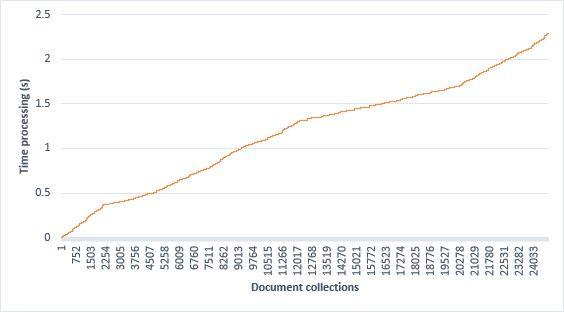
\includegraphics[scale=1]{timeProcessingInvertedIndex}
	}
	\caption{Time processing document collections into inverted index.}\label{fig:timeProcessingInvertedIndex}
\end{figure}

Processing documents and input into virtual museum inverted index for 24.608 collections require processing time approximately 2.29 seconds by using Intel Xeon Processor 2620v4, memory DDR4 32Gb, and Kingston Savage SSD 256Gb. This index intends to be used for serving all user’s activities in front end server. Further, this inverted index has tested by using query document to document as this research main goal to approximate thematic collections related to user’s activity and document collections.

\begin{figure}[ht]
	\centerfloat{
		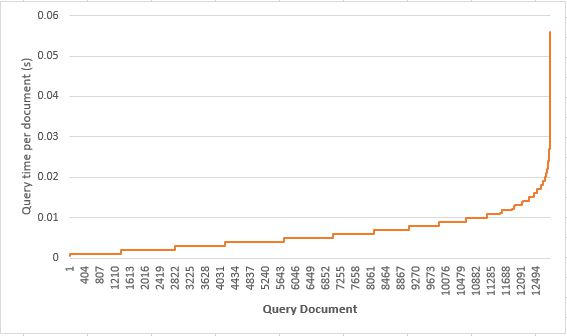
\includegraphics[scale=1]{timeProcessingDocumentQuery}
	}
	\caption{Elapsed time processing document to document query.}\label{fig:timeProcessingDocumentQuery}
\end{figure}

The result in Fig.~\cref{fig:timeProcessingDocumentQuery}, show that given a query “a document to a document” require time less than one microsecond per query, this is aligned with the main goal to design virtual museum inverted index data structure to serve more fast and relevant.

\subsubsection{Visulization}
\paragraph{A. Collections in Map}
Information visualization is one of concern in thematic exhibition in order to deliver and serve high quality experience to the visitors.
Design map plan and leveling will help visitors to classify information which has previously received from information traveling visualization. Let visitor move to the area inside the map which could be formed to the internal or external exhibition with there are no predefine items have assigned. Providing more space as a proportion to give object transformation is considerable as part of esthetics. The room design maybe contains object on the floor, wall or in some neared-location or can be reached by users as shown in Fig.~\cref{fig:designExplorationRoom}.

\begin{figure}[ht]
	\centerfloat{
		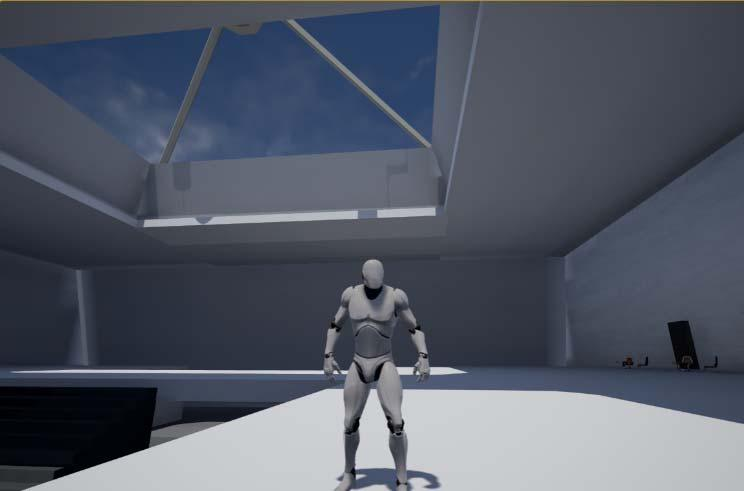
\includegraphics[scale=1]{designExplorationRoom}
	}
	\caption{Design Exploration Room for Collection Exhibition.}\label{fig:designExplorationRoom}
\end{figure}

Give the floor planning with good navigation will make users easier to use this system. In virtual it can be providing area by grouping the object, even this particular area didn’t exist on the real museum institution.

\paragraph{B. Dynamic Collection Visualization}
When the users visiting a virtual museum, the system should determine what is the information trying to convey? what the motivated topics which make them enjoy and satisfied? In this situation, thematic virtual museum trying to create the system to maintain interactive information. The collections will appear after automatic user query have been processed. The exhibition which has been displayed should be drawn users’ attention and make more attractive by triggering with relevant collections visualization.

The degree of similarity will be leading user from room to room or an area to area of exhibition as shown in Fig.~\cref{fig:dynamicCollectionsArea}. It can be pre-labeling data as a temporary or a permanent exhibition for each object in spread area. The system will be responsible for redisplaying contents by marking user traversed area.

\begin{figure}[ht]
	\centerfloat{
		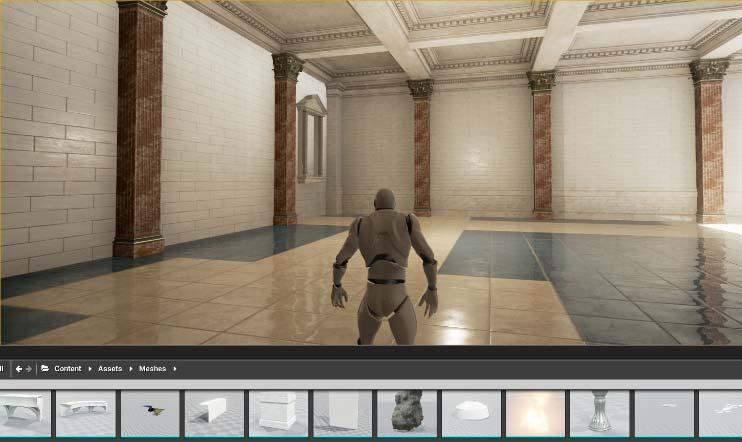
\includegraphics[scale=1]{dynamicCollectionsArea}
	}
	\caption{Dynamic Collections Area.}\label{fig:dynamicCollectionsArea}
\end{figure}

Creating specific functional area design for scheduled thematic event exhibition is recommended to perform flexible objects which have determined include newly arrived collection in some museums. Along the process, user respond and time spent in the room or area where collections appeared must be recorded as a feedback parameter. User also can be projecting some group of collections base on a manual query to the system with or without their base information.

The dynamic collection will collect visitor visit experiences in order to be processed near real time or next time when visitors will come back again on this system. Trying to understand the visitors to far and more complex by defining some variables is very useful in background inverted index process. Quantitative measures such as demographics provide too little information about visitors in relation to museums to be a useful variable for describing and understanding the museum visitor experience \cite{Falk}.

\paragraph{C. User Interaction}
User interaction always recorded by the system on the fly and this information in near real-time will be automatically processed in the background. The result of those process will generate more accurate information related to visitor characteristics, behavior and desire. Defining embedded information into inverted index is helpful for delivering more accurate exhibitions in the specific fields.

When users are walking around the space, the system provides a feature to control some object which has an ability to be controlled, this approach is mean to increase user sensitivity and reaction to gain new knowledge or discovery. Design direct or indirect appearance of the objects can be projected over a period of time. Understanding user needs and wants is critical for exhibition space to be not only attractive and effective for display but also accessible \cite{LordPiacente}.

Working to design ideal interface to the end-user is very crucial things, affected visitor will return another time if visitors satisfied using the application or will be leaving because some of poor user interface design, those all approximation for design user interface visualization.

\subsubsection{Conclusion and Future Work}
In this paper showed a design and modification of the inverted index experimental result for thematic virtual museums system and a sample of exhibition visualization to get more precision by embedding method. This research will continue to implement this index from contextual to concept by using latent semantic indexing (LSI) projection in future work and improving user interface for more attractive.

\subsection{Design Muntoi web-based framework and search engine analytics for thematic virtual museums}\label{subsec:ch4/sec2/sub3}

\subsubsection{Introduction.} The future development of virtual museum focused on the exhibition of the collections which contained in databases of museum institutions, based on the information from this collections, curators can design virtual exhibition, environment, game, and simulation in 3D, panoramic 360 degree and also it will help them to expand access to the collections through sophisticated platform.

To realize this kind of idea, we are providing attractive, effective, and interactive user interface, which giving the user more experiences and having fun when they accessing the system. The currently platform which the most widely used and easily accessible by the user is website. Therefore it is necessary to design a framework that can serve needs of the user, low-cost and aligned with the concept of thematic virtual museums.

The design is adopting the concept of Model-View-Controller (MVC) which widely used in the web-based framework where it can simplify developer to create a structured application, making application maintainable, extensible, easy to reuse code (efficient), and will be helping developer to build a program very fast. This framework will ensure consistency, separating logic and presentation layer. In addition the program also will be designed to be closely linked with the role of search engine analytics as a core program of thematic virtual museums.

\subsubsection{Research Objective.} The purpose of this research paper is to inform our progress on development of a web framework based on Go language to provide detail museum information, managing museum collections information, and design a concept of thematic virtual museum for attracting more visitors and design search engine analytics to become a core of the future development of virtual museums.

\subsubsection{Web Framework.} Web is the most powerful platform to handle time, distance and space limitation in physical museum institutions. Based on recent web technology, we have been designed web pages more responsive, interactive and dynamic.

Web framework is designed to develop dynamic website which have a good structure, providing common library, URL mapping, session and security again attacker, database manipulation, template to generating textual output, light- weight, and often providing concept Model-View-Controller (MVC). It is designed to make developer easier and faster for creating a website especially when they want to create scalable, maintainable and sustainable website.

Thematic virtual museums system has been developing based on Go Language web programming because we are pay for attention to the performance. A language which suitable for modern computing infrastructure, light on the page, good on networking and multiprocessing. Go aims to combine the safety and performance of a statically typed compiled language with the expressiveness and convenience of a dynamically typed interpreted language. It also aims to be suitable for modern systems programming \cite{Pike}.

The application has been using non-relational databases MongoDB for managing and maintaining collections information. This web framework, we call it \textit{Muntoi Framework (MuntoiFr}). The structure of \textit{MuntoiFr} as shown in Fig~\cref{fig:muntoiWebFramework}.

\begin{figure}[ht]
	\centerfloat{
		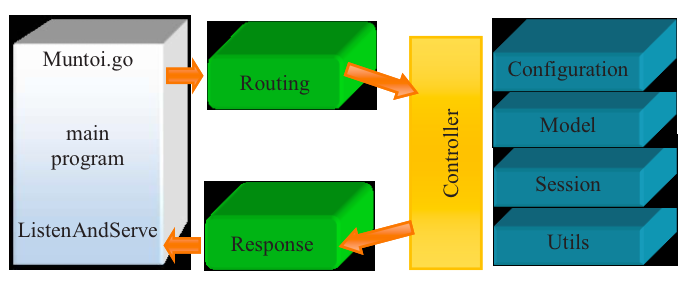
\includegraphics[scale=0.5]{muntoiWebFramework}
	}
	\caption{Structure of Muntoi Web Framework based on Model-View-Controller concept.}\label{fig:muntoiWebFramework}
\end{figure}

Server of virtual museum by default running on port 8080 which defined by developer inside main program \textit{(the source-code inside a file: Muntoi.go)}, this program will be handling http connections from client trough \textit{ListenAndServe} function that has provided by Go Language in the http package. We have created a routing for managing each request on the server by accessing web page, the routing table must be registered first by developer, it is intend to validate http request, matching uniform resource locator (URL), to ensure that requested-pages already defined on the server-side, and making request more safe and secure.

The controller is a specific function which responsible for scripting, organizing program code, logic, and then wrap the result to presentation layer. It is allow the program connecting and interacting to \textit{Model} that provide mapping persistence data layer. In controller we are parsing files as templates (HTML, CSS, JavaScript, etc.) to be rendered in View layer as output response, which visitors can interact to the system.

\textit{Model} is a mapping for data especially to handle information in our databases. In \textit{MuntoiFr} we are using MongoDB as main databases. MongoDB represents JSON documents in binary-encoded format called Binary JSON (BSON) behind the scenes. BSON extends the JSON model to provide additional data types and to be efficient for encoding and decoding within different languages, BSON implementation is lightweight, fast, highly traversable, and supports embedding objects and arrays within other objects and arrays \cite{JSONBSON}.

In general purpose \textit{MuntoiFr} is providing a script \textit{Configuration}: to define variables as initial values before the program will run on the server, \textit{Session}: to store temporary information on the server-side during a period of time which could be used across multiple pages, this feature always used for user authentication and validation, and \textit{Utils}: as a tool that contains several useful functions to perform certain in specific operations. \textit{MuntoiFr} have designed dynamically for model persistence therefore latter on it would be porting to another databases software without changing the structure of this framework.

\subsubsection{Design.} This system was developed using the concept of thematic virtual museums that one of its functions is connecting the museum collections information which interrelated each other. It is intended to help visitors to find something interesting and unique as they wish.

\begin{figure}[ht]
	\centerfloat{
		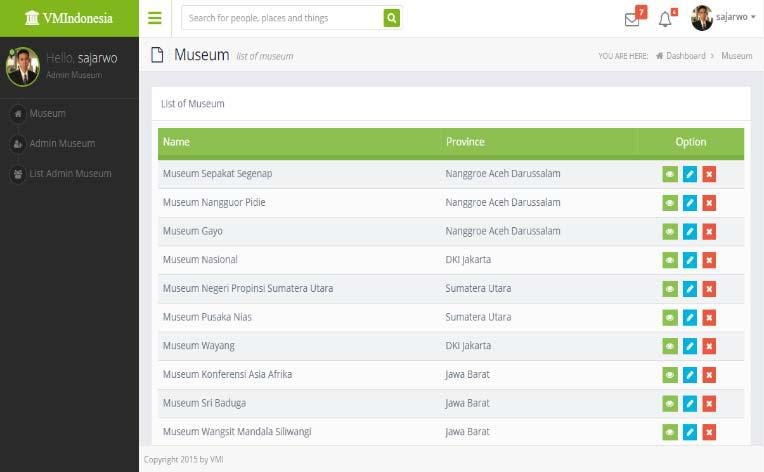
\includegraphics[scale=1]{designAdminPage}
	}
	\caption{Design administration page on the virtual museum web-based framework.}\label{fig:designAdminPage}
\end{figure}

Visitors are expected can appreciate the meaning and value of the collection that have been displayed with the help of this thematic virtual museum. The program could motivating and make visitors more comfortable and focus in learning, especially for students and researchers because the system providing information that related to their criteria and desires. This is as complement for reaching the future of museum to provide a personalized learning environment to support learning process \cite{Anggai}.

In order to manage museum institutions and collections information, we have created user authentication privileges as super-admin and admin for each museum institutions. User management page for assign access to the specific museum institution as shown in Fig.~\cref{fig:userAdminPage}

\begin{figure}[ht]
	\centerfloat{
		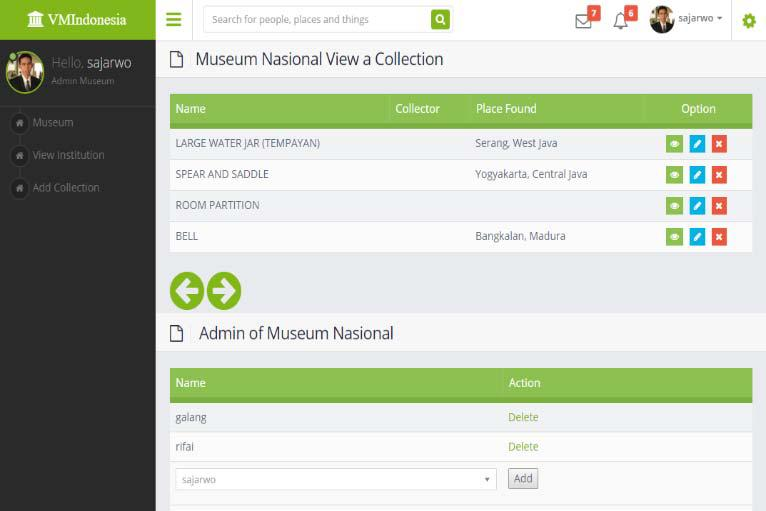
\includegraphics[scale=1]{userAdminPage}
	}
	\caption{User administration to assign privileges for specific institution on the virtual museum web-based framework.}\label{fig:userAdminPage}
\end{figure}

\textit{Super admin} rule can create, edit and remove list of museum institutions, collections and users. The museum administrator which have assigned can add museum collections, full with specific information on the form \textit{Register a Collection} such as name, collector, places found, date and period.

\begin{figure}[ht]
	\centerfloat{
		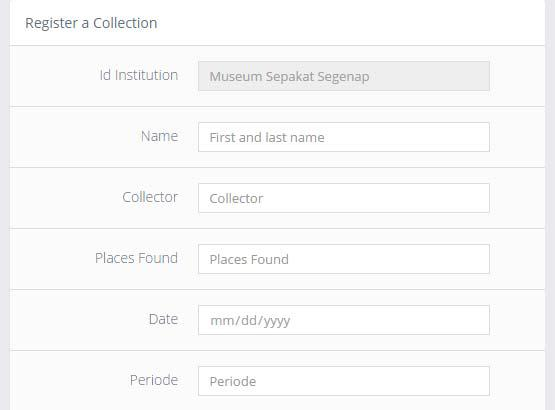
\includegraphics[scale=1]{museumForm}
	}
	\caption{Registration of the museum collections form.}\label{fig:museumForm}
\end{figure}

On the form \textit{Additional Information} contains: dimensions, weight, material, condition, total collection, date recorded which automatic filled at the present and description field for the information which still not covered yet in the previous fields. It also could be added another fields or specific form to enrich information which aligned with structure in database of MongoDB.

The thematic virtual museums programs focused or depend on information of each collections which are given or provided by several museum institutions.

As long as they know something about the category of objects and thus about the structure of the display, then a few glances may suffice to check off a few points, to stimulate thought, to supplement knowledge and more important, it provides information that has not been filtered out through these traditional methods \cite{Schweibenz}.

\begin{figure}[ht]
	\centerfloat{
		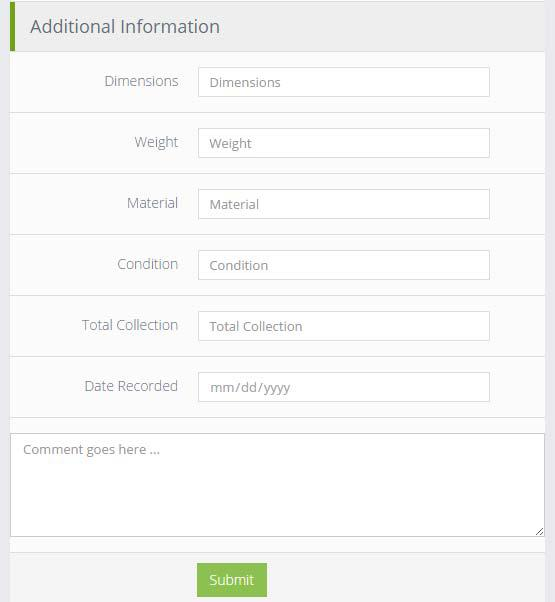
\includegraphics[scale=1]{additionalInfoForm}
	}
	\caption{Additional information form.}\label{fig:additionalInfoForm}
\end{figure}

Collections which contained in the system are automatically processed into a full information, inter-related each other and could be disseminating to all over the world through variety of media. This method will help for reducing cost of publication at museum institutions.

Nowadays sustainability become trending topic in Indonesian museums, which transforming or changing form traditional to modern. One of the focus discussion is the content. Content is very determining the existence of virtual museum, without good packaging content then the visitors will not be interesting to visit into the system. Complex information divided into small parts or synthesised. We cannot loose time in standing in front of an object, for example, for a long period. Museums need to communicate and to attract more visitors. The idea of a museum, whose goal is just the preservation or study of its collection, is no longer feasible \cite{Pescarin}.

In this system, we are providing comment from the visitor perspective to enrich base information, because recent technology allowing non museum professionals are now being invited to create their own input into museum collections and exhibitions. This method is known as user-generated content (UGC) \cite{HellinHobbs}.

In the future development process, thematic virtual museum will be built on two sides they are from curator and visitor side. Curator will be able to provide or display a visualization of interactive contents and exhibitions with the help of analytics software that will be integrated in this framework.

As our work in development of Virtual Museum in Indonesia as instrumental for supporting the achievement of the museum functions as a whole and using social media to campaign collections, broadcast contents based on their location, communicating with visitor, attract and influence society, exchange information and waiting for their feedback from user perspective to improve public services \cite{AnggaiBlekanovSergeev2014}, we are designing search engine analytics for thematic virtual museum as show in Fig.~\cref{fig:searchEngineAnalytics}.

\begin{figure}[ht]
	\centerfloat{
		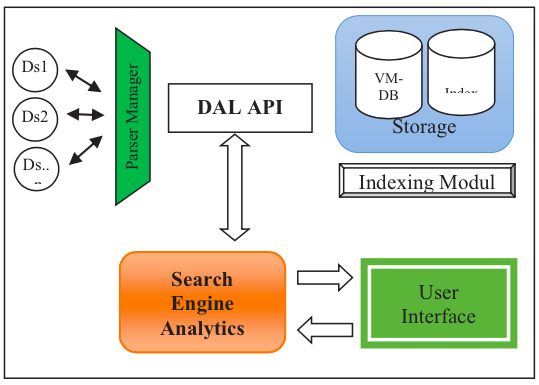
\includegraphics[scale=0.5]{searchEngineAnalytics}
	}
	\caption{Search Engine Analytics as a core program based on the concept of Thematic Virtual Museums.}\label{fig:searchEngineAnalytics}
\end{figure}

Thematic virtual museum will be providing Data Access Layer (DAL) or Application Programming Interface (API) for integrating and accessing data sources in museum institutions. This engine working to extracting and obtain relevant information from data sources, designing to understand structure data in current database or semantically tagged of museum institutions where they used to store collections information, and system also support to manage unstructured data that have not define data-model or semantic \cite{AnggaiBlekanovSergeev2014}. We are using indexing modules in order to process data or information, and some of them will be stored into the general VM-Databases as a base of information. DAL also will be serving an access on \textit{FrontEnd} in which User Interface can leading early query to Search Engine Analytics.

Parser manager will be used to parsing all data resources from museum institutions and return an output into structured form. In this early stages, data or information can be classified before this information will be delivering to VM-Databases or indexing module. Parser manager have to know protocol or standard for data integration for grabbing sources information inside museum institutions.

Search Engine Analytics task is responsible to find themes of the museum exhibition, and a unique collection to be displayed, based on the information inside the museum institutions which intersect with visitor characteristics, behaviours and desires. The concept of this analytics also designed to find possibility to build thematic exhibitions from permanent collections, following a narrative approach to enhance visitor experience and knowledge \cite{Pescarin}.

Analytics Engine will be designed to processing and simplify the information before delivering it to the specific visitor. This engine also will help for campaign collection, not only display most necessary information but also provide better interrelation between the museum collections at the different institutions. We believe that in the museum institutions especially in Indonesia have many similarities information of the each object collections which if we treated properly using the analytic engine as a tool, it will be leading curator and researcher to a new history that has not been revealed yet.

Smart system in the application of thematic virtual museum will automatic adapting, recording all user activity, perceptions and responses as part user experience before, during and after they used the virtual museum services. This feature is an important part to ensure and determine how the system can formulate in order to retrieving closely information from data source,and generating best-result to the visitors. It is leading to develop a system for extracting and processing data sources until become important information and useful for visitors \cite{AnggaiBlekanovSergeev2014}.

Our approach will focus on displaying closest information to the visitor trough real map navigation inside the museum institutions, timeline of the collections itself and another one as Tilman et al. approach is the content itself to build a path. Both approaches have in common, that the user can stroll digitally to encounter unexpected information and users can stroll in the exhibit rooms freely because the information units can be combined in any constellation possible \cite{DeuschelHeussHumm}.

The Search Engine Analytics with thematic approach will be designing to provide and construct the relevant information in order to displaying content in 3D model to become more interactive. The interactive 3D model enables the user to interact with the object, turning it around and exploring its details. This is also not possible in the physical museum. Rizvic stete that the story was the main distinguishing factor and its existence motivated users to visit more exhibits in virtual museum therefore the environments will be implemented as pre-rendered images with hotspots, instead of real time 3D environments \cite{Rizvic}.

Through thematic virtual museums system, some information topics/theme which have been sorted and formulated by curator can be used as exhibition. In general exhibitions in virtual museum for attracting visitor will be presented in 3D environments which can have a stronger cognitive impact, as they give learners the feeling of being in the simulated reality, thus improving the understanding and memorization of the information \cite{GheorghiuStefan}. However, not all objects in real museum can be presenting in 3D model, it is depend on the form and default information attached to the object itself.

\subsubsection{Conclusion and Future Work.} In this paper, we have informed our progress about development web-based framework using Go Language for thematic virtual museums and concept and design of Search Engine Analytics as a core of this system to provide closest information to the visitors.

In future work, we intend to continue this research and will develop Search Engine Analytics based on the approach of thematic virtual museum which can be used to process data or information inside museum institutions.

\subsection{Management and information processing at virtual museum}\label{subsec:ch4/sec2/sub4}

\subsubsection{Introduction.} Almost every country have their own museum and standard procedure with different characteristics based on their state policies. In Indonesia itself until now, there are approximately 300 museum institutions under Ministry of Education and Culture (MOEC), Republic of Indonesia (RI) and Private Corporation. The government state about \textit{Gerakan Nasional Cinta Museum} (GNCM) or national movement of museum lover, through Visit Museum Year (2010-2014) program. GNCM intend to strengthen three main pillars of the museum in Indonesia, namely 1) educating the nation, 2) forming personality (character) of the nation, and 3) embed the concept of national resilience and insight on archipelago \cite{MunandarPerdanaRahayu}.

According to the International Council of Museum (ICOM) statutes, adopted during the 21st General Conference in Vienna, Austria, in 2007: A museum is a non-profit, permanent institution in the service of society and its development, open to the public, which acquires, conserves, researches, communicates and exhibits the tangible and intangible heritage of humanity and its environment for the purposes of education, study and enjoyment \cite{DesvaleesMairesse}.

Museum architecture as the art of designing and building a space that will be used to house specific museum functions, more particularly the functions of exhibition and display, preventive and remedial active conservation, study, management, and receiving visitors. Museum buildings was often focused on safeguarding collections, even they created storage areas by creating space in the basement, or by building new structures \cite{MunandarPerdanaRahayu}. In other word, museum is the only place to store the collections and not at all of museum’s collections were displayed.

There are many problems currently faced by the museums include the management and processing data collection either structured or unstructured inside the institutions. Therefore, this research was undertaken in processing and managing data in the museum institutions in order to be delivered to the public based on customized information they need.

\subsubsection{Research Objective.} The purpose of this research are to identifying, investigating the real problem in physical and management at museums, how they spread information in digital era and how to design a virtual museum system in retrieving information from structure and unstructured data related to the collections information.

\subsubsection{Investigation.} 
For strengthening our research, currently we have investigated Museum of Geology, National Museum in Indonesia has a total collections more than 141.899 items, consists of seven types of collections are prehistoric, archeology, ceramics, numismtik-heraldic, history, ethnography and geography \cite{IndonesiaMuseum}, Hermitage Museum in Russia, and for balancing we also observe online resources provided by Louvre Museum in France and Virtual Museum of Canada (VMC) to enhance Canadians’ knowledge, understanding and appreciation of events, experiences, people and objects that reflect and have shaped Canada’s history and identity. VMC providing more than 500 virtual exhibits promoting the content of Canadian museums, 150 interactive resources, over 365 learning resources including lesson plans and educational activities. VMC content provided by many collaborator approximately 1,600 museums \cite{CanadaMuseum}.

We have founded many problems at the museum institutions, which are classifying as the following:

\paragraph{A. Physical} Museum institution in general providing physical access to museum environment and it resource as a part of public services, but in our investigation there are lack of the physical museum, they are:
\begin{itemize}
	\item Time limitation, visitation to the museum is limited to the visitors.
	\item Distance limitations, visitor could not be attending to the museum because too far away from their hometown, separated by island, country or continent.
	\item Space limitation for exhibition, therefore not all collections displayed at the exhibition room, and they put the collections on storage area.
	\item Museum with many rooms will make visitor confuse, and sometime visitor do not want to see a specific collection because of phobia or not meet with visitor desire.
	\item Collections information provided by museum institution usually are not detail, therefore visitors do not understand the collection he saw and did not enjoy his visit.
	\item Communication among visitors wore not happened, at the end it happen only from guide to visitor or vice versa.
	\item Not all people know the existence of museums and their object collections.
\end{itemize}

\paragraph{B. Management} Management in museum have been facing many problem as follows:
\begin{itemize}
	\item Museum institution have big object data collections, some of them still on process to classify and identify by researcher.
	\item Data in the museums ware separated and become hard to maintain.
	\item Object collections can be lose or broken because of natural disasters (force majeure).
	\item Lack of museum publicity, imaging, promotion and service include informing an event will providing by the museum institution.
	\item Community, observer and lover of museum has not been established. Even the government state about National Movement of Museum Lover, through Visit Museum Year (2010-2014).
	\item Implementation and management of the museum is not in line with recent development of information technology.
	\item Online information, some of the museum have websites, but they are limited and only provide information about the museum institution and not the object collections.
	\item Information for tourism or researcher from other country still not provided by museum institution.
	\item Route and destination for best way to visit the place still not established yet. Route and destination information are very important for tourist and local to find the best way, reducing cost and time.
	\item Mobile technology with virtual guide still focus on highlight catalogue, news, and floor plan, but they forget to provide floor plan with direction to each room which providing collection information that meet with visitors desire.
\end{itemize}

\subsubsection{Concept and Design}

In general museum institutions have many data and information of object collections, some of them have a complete documentation and the other just a half or even minor of information. The collections usually displayed at exhibition room and the other at storage area with full access or restricted. Museum visitor visiting museum, observing the collection and back to home with or without information.

Museum visitors come to see and observe a variety of collections that were displayed by museum, but what they see perhaps not necessary meet with their criteria, desires and preferences of the visitors itself.

Until now, museum institution for providing public services try to attract visitors with developing audio-visual, make visitors comfortable to surfing and searching information of the collections and exhibition through their website with 2D or 3D visualization as shown in Fig.~\cref{fig:virtualMuseumCanada}.

\begin{figure}[ht]
	\centerfloat{
		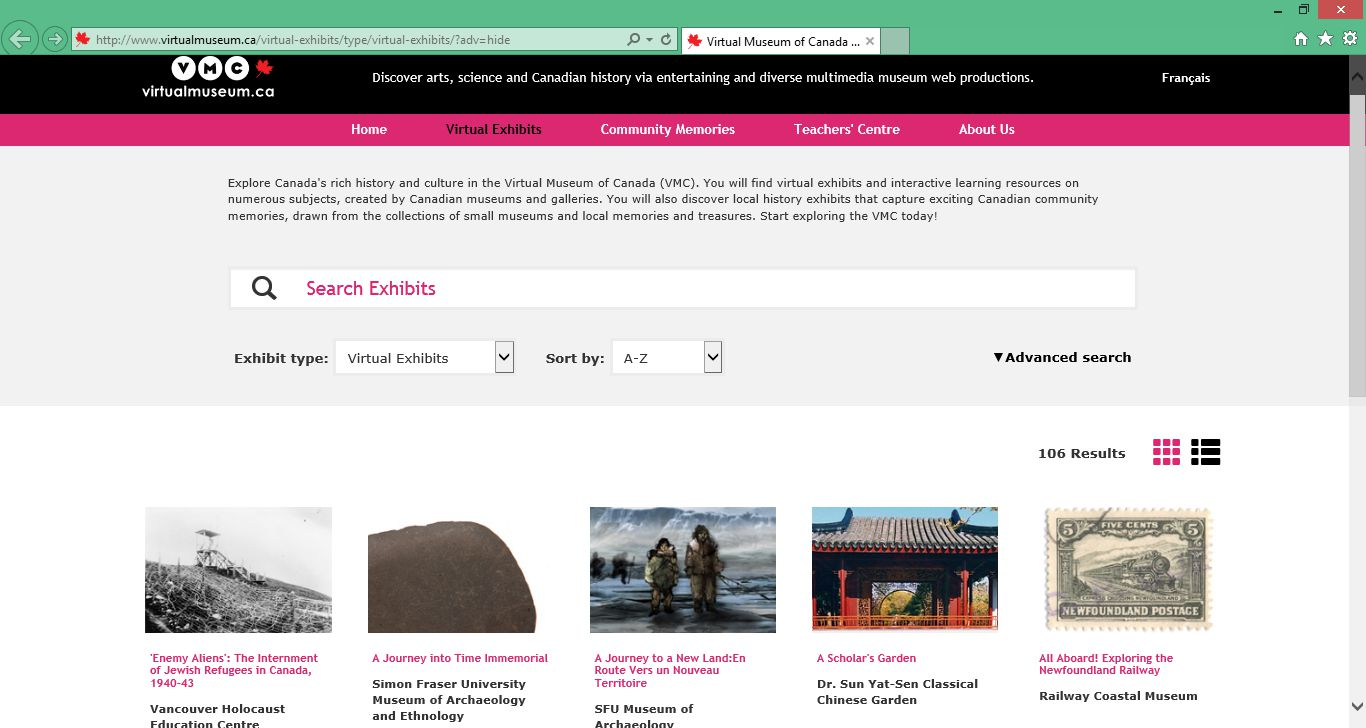
\includegraphics[scale=1.0]{virtualMuseumCanada}
	}
	\caption{Website of Virtual Museum of Canada providing exhibition in cyber space.}\label{fig:virtualMuseumCanada}
\end{figure}

Information delivered through website as in Fig.~\cref{fig:virtualMuseumCanada} focus on one subject exhibited and VMC website also providing services for searching collection information, but unfortunately when visitor found a collection, the system only describing about the collection itself and not related to similar collection inside 1,600 museums managed by VMC.

While VMC providing information through website, Hermitage Museum in Saint Petersburg, Russia providing application in mobile devices as a guide for the visitor in 5 languages, include floor plan, news, collection and catalogue as shown in Fig.~\cref{fig:hermitageApp}.

\begin{figure}[ht]
	\centerfloat{
		\hfill
		\subcaptionbox[List-of-Figures entry]{\label{fig:hermitageApp-1}}{%
			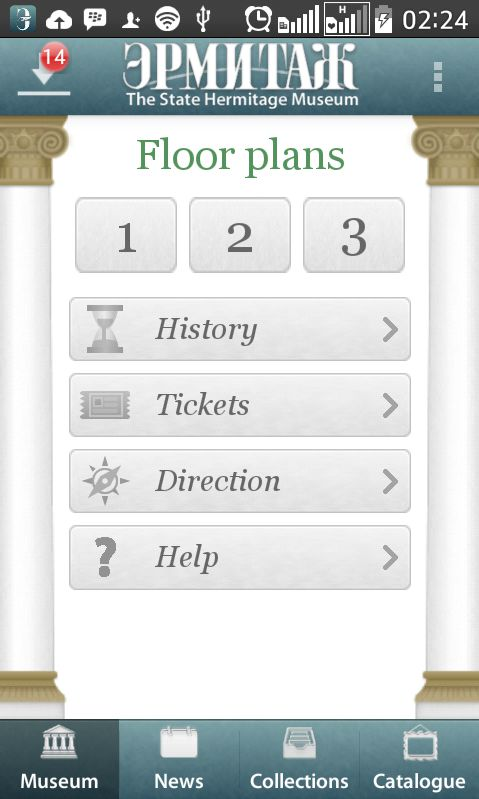
\includegraphics[width=0.3\linewidth]{hermitageApp1}}
		\subcaptionbox{\label{fig:hermitageApp-2}}{%
			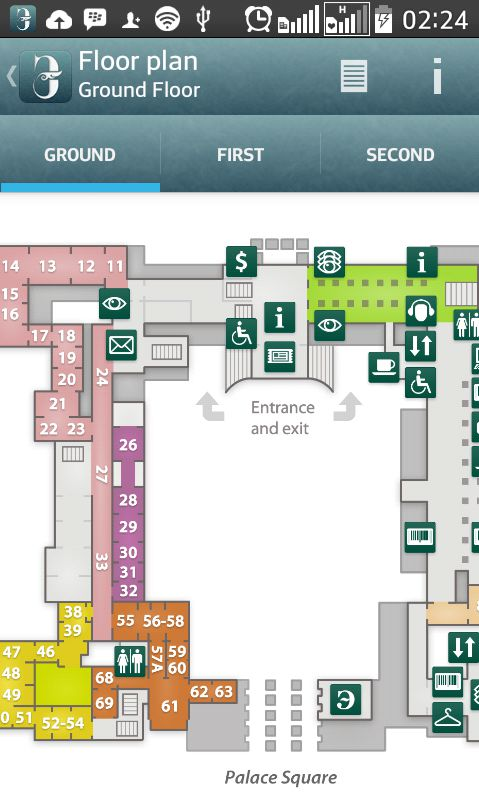
\includegraphics[width=0.3\linewidth]{hermitageApp2}}
		\subcaptionbox{\label{fig:hermitageApp-3}}{%
			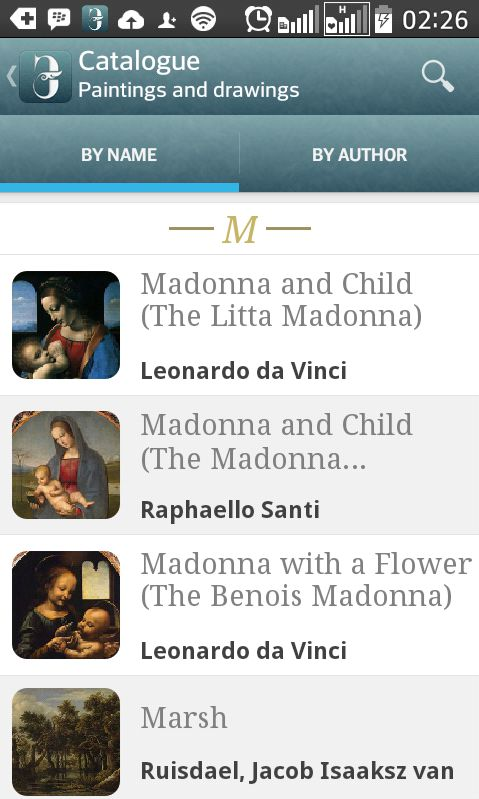
\includegraphics[width=0.3\linewidth]{hermitageApp3}}
		\hfill
	}
	\caption{Mobile Application provided by Tour Bureau of the Hermitage Museum, Saint Petersburg, Russia.
	}\label{fig:hermitageApp}
\end{figure}

Museum of Geology and National Museum are providing website but just for general information and not focused on exhibition and collection. In Museum Geology we have founded many data related to the collection and they try to documenting, recreate numbering system for each object, some of collection information indeed not discovered yet (researcher still working to identify the object collections), and the other information still based on old paper report. Recently they managing all collections in exhibition room and storage area and saving the information inside internal database application as shown in Fig.~\cref{fig:dbMuseumIndonesia}.

\begin{figure}[ht]
	\centerfloat{
		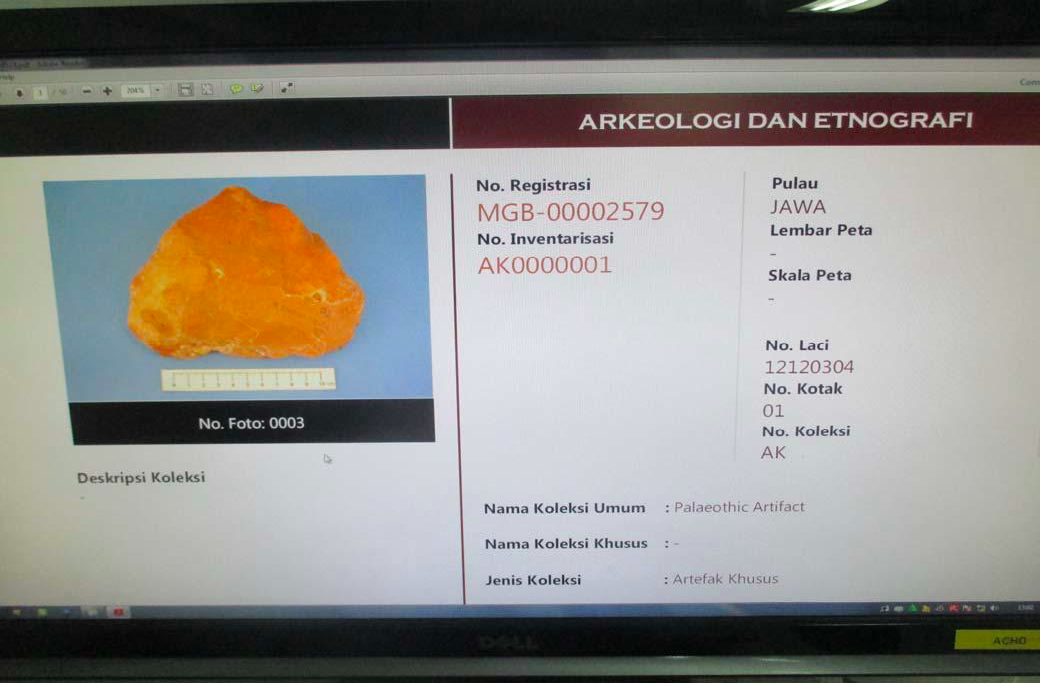
\includegraphics[scale=0.3]{dbMuseumIndonesia}
	}
	\caption{Collection databases for internal management in Museum of Geology, Indonesia.}\label{fig:dbMuseumIndonesia}
\end{figure}

National Museum official website providing eye catching collections not more than 100 collections, and if visitors want to see the collections have been displaying in National Museum through website, of course they will not find all collections including those in storage area. The other featured collections they put on Google Art Project website to promote the artwork as shown in Fig.~\cref{fig:museumGoogleArt}.

\begin{figure}[ht]
	\centerfloat{
		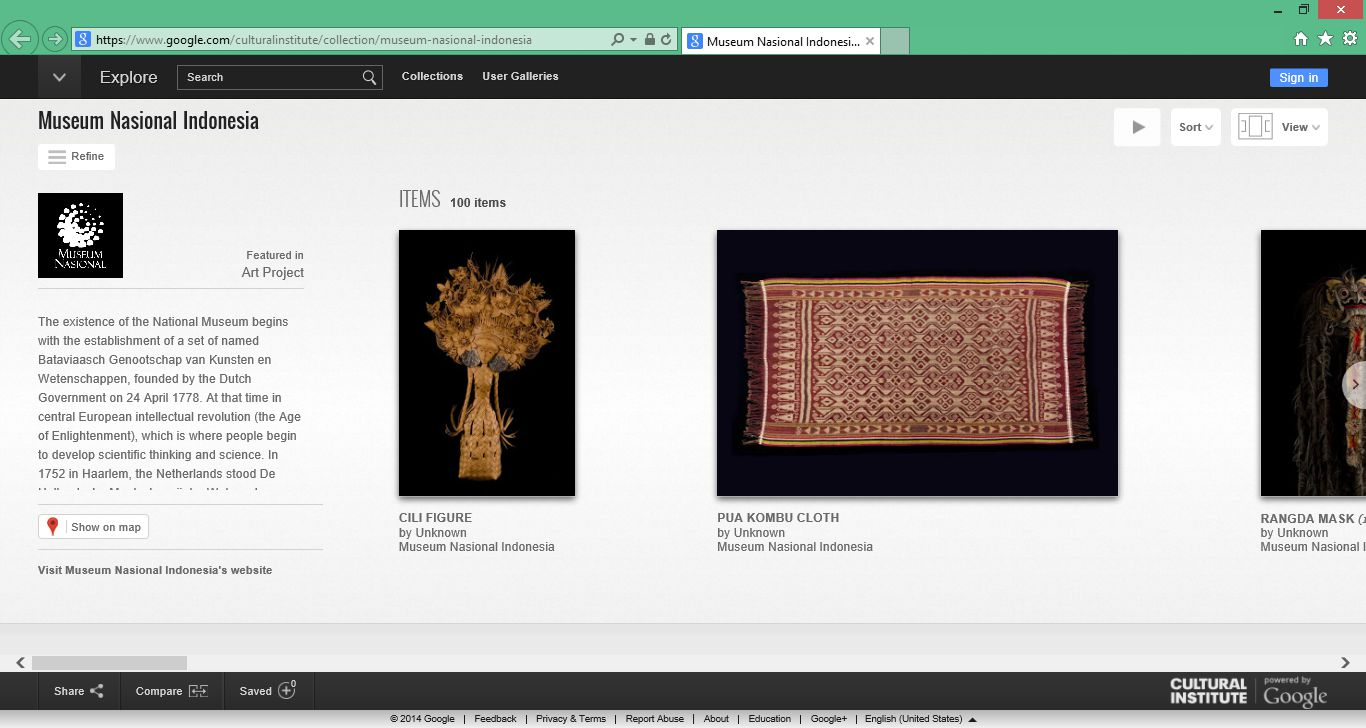
\includegraphics[scale=1.0]{museumGoogleArt}
	}
	\caption{National Museum program for promoting artwork through Google Art project website.}\label{fig:museumGoogleArt}
\end{figure}

The information system between Museum of Geology and Museum National are not connected include featured collections in Google Art, therefore there is no linkage information on the collections of both institutions despite the fact that there is a closely interconnected collections information in both institutions.

In this situation and condition, museum institutions in Indonesia must be find alternative solution for solving the problems both in the exhibits and collections. One proposing solution in digital age is developing Virtual Museum in Indonesia as instrumental for supporting the achievement of the museum functions as a whole and using social media to campaign collections, broadcast contents based on their location, communicating with visitor, attract and influence society, exchange information and waiting for their feedback from user perspective to improve public services. According to Steve Dietz, et al, in the book The Next Generation of Virtual Museum include: integrated with social media to share experiences and knowledge \cite{Dietz}.

The design of system also cover cyber exhibition program, and linked with source of collection information in each museum institutions both internal and external uses. Lia Laela in her thesis stated that cyber exhibition developed as a complement of the exhibition held in the real museum, not as a replacement. The system had tested to the several users and the results show that users get different and more interactive experiences and detailed information compared to what they get when visiting the physical museum. The cyber exhibition also add values to the collections, therefore they become more meaningful \cite{Sarah}. Virtual museum designed as a part of the future of museum that integrates with social networking in the process of collection and dissemination of information supporting the existence of good communication between the visitors and trustees of the museum in cyberspace. The future of museum provide a personalized learning environment to support learning process \cite{Anggai}.

Virtual museum system will be providing easy way to conduct learning process through cyber exhibition, whatever topics related to the collections will be presented to the user as possible. Learning process at cyber exhibition will be automatically happening when the visitors accessing the virtual museum system. The system will providing right information and also showing related information for assisting visitors to explore into deep substance of the information. Yeni in her paper try to integrate discovery-learning method into virtual museum. There were increased cognitive learning outcomes after students learning through discovery-learning method. This is the early start to realize virtual museum as the concept development of future museum \cite{Nurhasanah}.

Smart system in virtual museum will automatic adapting, record all user activity, perceptions and responses as part user experience before, during and after used virtual museum services. This feature is an important part to ensure and determine how the system retrieving closely information from data source to the visitor. Ratri stated that problem related to interactivity is a lack source of the visitors' learning experience. The teaching learning process conducted in museums generally covers listening, visualization, or visualization and listening area. One of the ways to handle the problems is to develop web based virtual museum because it will increase student’s motivation and could be accesses wherever and whenever as long as computers and internet connection are available \cite{Kayungyun}. The system will be designed to understand user, and meet with their expectation through data visualization in variety prospective.

Each collection in museum institutions have structure and unstructured data source. This data sources increase day by day and become hard to maintain, therefore necessary to develop a system for extracting and processing data sources until become important information and useful for visitors as shown in Fig.~\cref{fig:virtualMuseumEngine}.

\begin{figure}[ht]
	\centerfloat{
		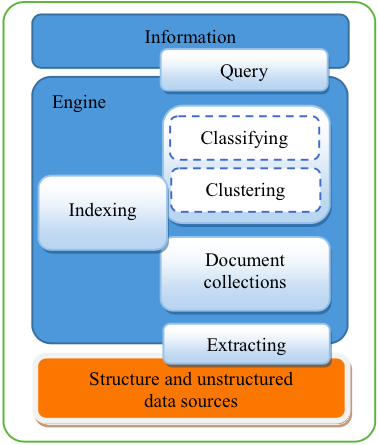
\includegraphics[scale=0.5]{virtualMuseumEngine}
	}
	\caption{How virtual museum engine extracting structure and unstructured data source to become important and relevant information.}\label{fig:virtualMuseumEngine}
\end{figure}

In Fig.~\cref{fig:virtualMuseumEngine} show how virtual museum engine working to extracting and obtain relevant information from data sources. The activity to retrieving information usually called information retrieval (IR). IR is finding material (usually documents) of an unstructured nature (usually text) that satisfies an information need from within large collections (usually stored on computers) \cite{ManningRaghavanSchutze}.

System will be designing to understand structure data in current database or semantically tagged of museum institutions where they used to store collections information, and system also support to manage unstructured data that have not define data-model or semantic. Result of extraction process are document collections which every document have unique numbering as identity (trough tokenizing process) before engine continue to the next step. For identifying language of the document we will prepare terms dictionary include stemming algorithm especially for Indonesian language (common language have been using as primary language of the resources that have been collected) to reducing term size. We will also preparing some algorithm for constructing static and dynamic index with compression in order to less disk space.

The system create classification for routing, filtering and segmenting, while clustering will be useful in grouping documents, because of this feature collections information are displaying to the visitor will automatically be closely linked with other collections. User interaction to the system also need to be translated into query with optimization in order to precise result of information needed. The system will formulate source of information therefore visitors can understand the object collections by providing detailed information and relevant to the object. Thus, visitors not only enjoy the view of the object but rather get a complete understanding. System that has integrated help of the mnemonic to the user in understanding the activity within the meaning of the value contained in an object of collection in virtual museum.

The benefit of applying method to retrieve information in museum for researchers are helping and assisting them by providing relevant information to the object of research in uncovering the meaning either before or after a visit to the stored object of collection in museum. Recent technology providing easy access to the source of information, therefore visitors can use a variety of media to access information residing in a virtual museum system as shown in Fig.~\cref{fig:visitorsAccess}.

\begin{figure}[ht]
	\centerfloat{
		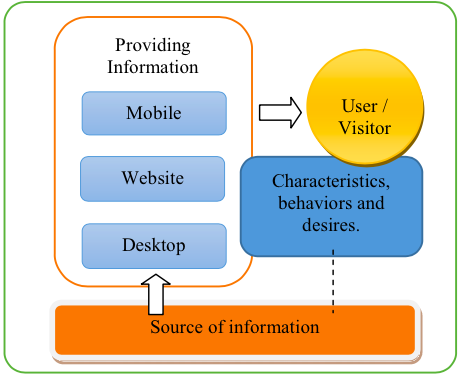
\includegraphics[scale=0.5]{visitorsAccess}
	}
	\caption{Visitor accessing source of information through variety of media which meet their characteristics, behaviours and desires.}\label{fig:visitorsAccess}
\end{figure}

In Fig.~\cref{fig:visitorsAccess} virtual museum as a complex system delivering an information to the user to answer necessary services for internal and external uses. In our investigation, virtual museum should know, determining, providing information based on visitors characteristics, behaviours and desires. Retrieving information for each collection and combining with user characteristics is need big resources, therefore we want to combine some algorithms in determining which one the best algorithm to solve the problem. This engine of virtual museum also could be uses as complement of teaching and learning onsite or through the distance where are visitor really know what they need to learn based on the materials and sources of collection information.

Task to provide information access will be handling by engine as a core system inside virtual museum. This engine have two tasks, first task is processing old to recently data sources in museum institutions as shown in Fig.~\cref{fig:virtualMuseumEngine}, and the second is handling users direct request to the information of collection itself, processing and delivering information need based on user characteristics, and acting as a real-time guidance as shown in Fig.~\cref{fig:virtualMuseumCanada}. The virtual museum system not only processing data sources to become important information, but also attracting visitors to the interesting places and give the right information of collections. In this case we assume that right information is not enough, therefore system need to process once more time the information to become closest information for the visitors.

\subsubsection{Conclusion and Future Work}

In this paper, we have investigated Museum of Geology, National Museum in Indonesia, Hermitage Museum in Russia, and for balancing we also observe online resources provided by Louvre Museum in France and Virtual Museum of Canada. Our result is a design of virtual museum engine which can obtain relevant information based on visitor characteristics, behaviours and desires through variety of media.

We intend to continue this work and develop a method for complements: the next generation of museum, cyber or virtual museum in the world. We also planning to improve this research to become a smart system which can be used in various areas for analyzing, processing, retrieving and delivering information.

\subsection{Modification biterm topic model input feature for detecting topic in thematic virtual museums}\label{subsec:ch4/sec2/sub5}

\paragraph{Introduction.} Recent year topic model is becoming a popular method to identify and organise hidden topic in document collections. The topic model can discover and determine latent topic from a large number of unstructured texts in a corpus automatically using bag of words techniques. In the virtual museum, a curator or museum administrator are analysing and organising numerous online exhibitions of museum object collections to communicate their existence, contextual, value, and many reasons behind the objects. However, they are relying on label information and metadata from the structured database for providing online or thematic exhibitions, and some of the museum institutions do not have thematic exhibitions \cite{Anggai,Foo,Champion,Palombini}.

In development latent information and discovering a topic from a document corpus, there are several techniques have been proposed such as latent semantic indexing (LSI) \cite{DeerwesterDumaisFurnas}, which offering dimensionality reduction using singular value decomposition and extended calculation from traditional vector space model (VSM). LSI has solved problems about a word or phrase that means exactly or nearly the same as another word or phrase in the same language (synonym) and the coexistence of many possible meanings for a word or phrase (polysemy). LSI also produces a representation of the underlying “latent” semantic structure of the information. Retrieving information in LSI overcomes some of the problems of keyword matching by retrieval based on the higher level semantic structure rather than just the surface level word choice \cite{Foltz}.

In 1998, Hofmann introduced unsupervised learning technique called probabilistic latent semantic indexing (PLSI) that had a solid statistical foundation. Since it based on the likelihood principle, defines a proper generative model of the data, identifying and distinguishing between different contexts of word usage without recourse to a dictionary or thesaurus \cite{Hofmann1999,Hofmann2001} it assumes that in the document contain topics mixtures. In 2003, David Blei et al., proposed latent Dirichlet allocation (LDA) \cite{BleiNgJordan}, which used the generative probabilistic model of a corpus and represented a mixture of topics in normal document texts. However, due to poor conventional topic models such as PLSI and LDA, Yan et al., proposed generative biterm topic model (BTM) \cite{YanGuoLan,ChengYanLan} to overcome short texts in a document, and this method outperform LDA even on normal texts.

In this research work, we conduct experiments to exploit BTM feature parameter by modifying input feature of third step BTM generative process in order to improve topic quality and discover themes from virtual museum document collections automatically.

\paragraph{Biterm Topic Model.} The BTM basic concept was generating biterm or word-pair from the whole corpus, where the word-pair co-occurrence pattern was an unordering from the fixed sliding window. The generated co-occurrence word from document sliding window and built a set of word-pair of the whole corpus made BTM enhanced topic learning and solved the problem of the sparse word at the document level. The data generation process under BTM had the result the corpus consists of a mixture of topics, and each biterm drew from a specific topic \cite{YanGuoLan,ChengYanLan}. The graphical BTM plate representation as shown in Fig.~\cref{fig:graphicalBTM} \cite{YanGuoLan}.

\begin{figure}[ht]
	\centerfloat{
		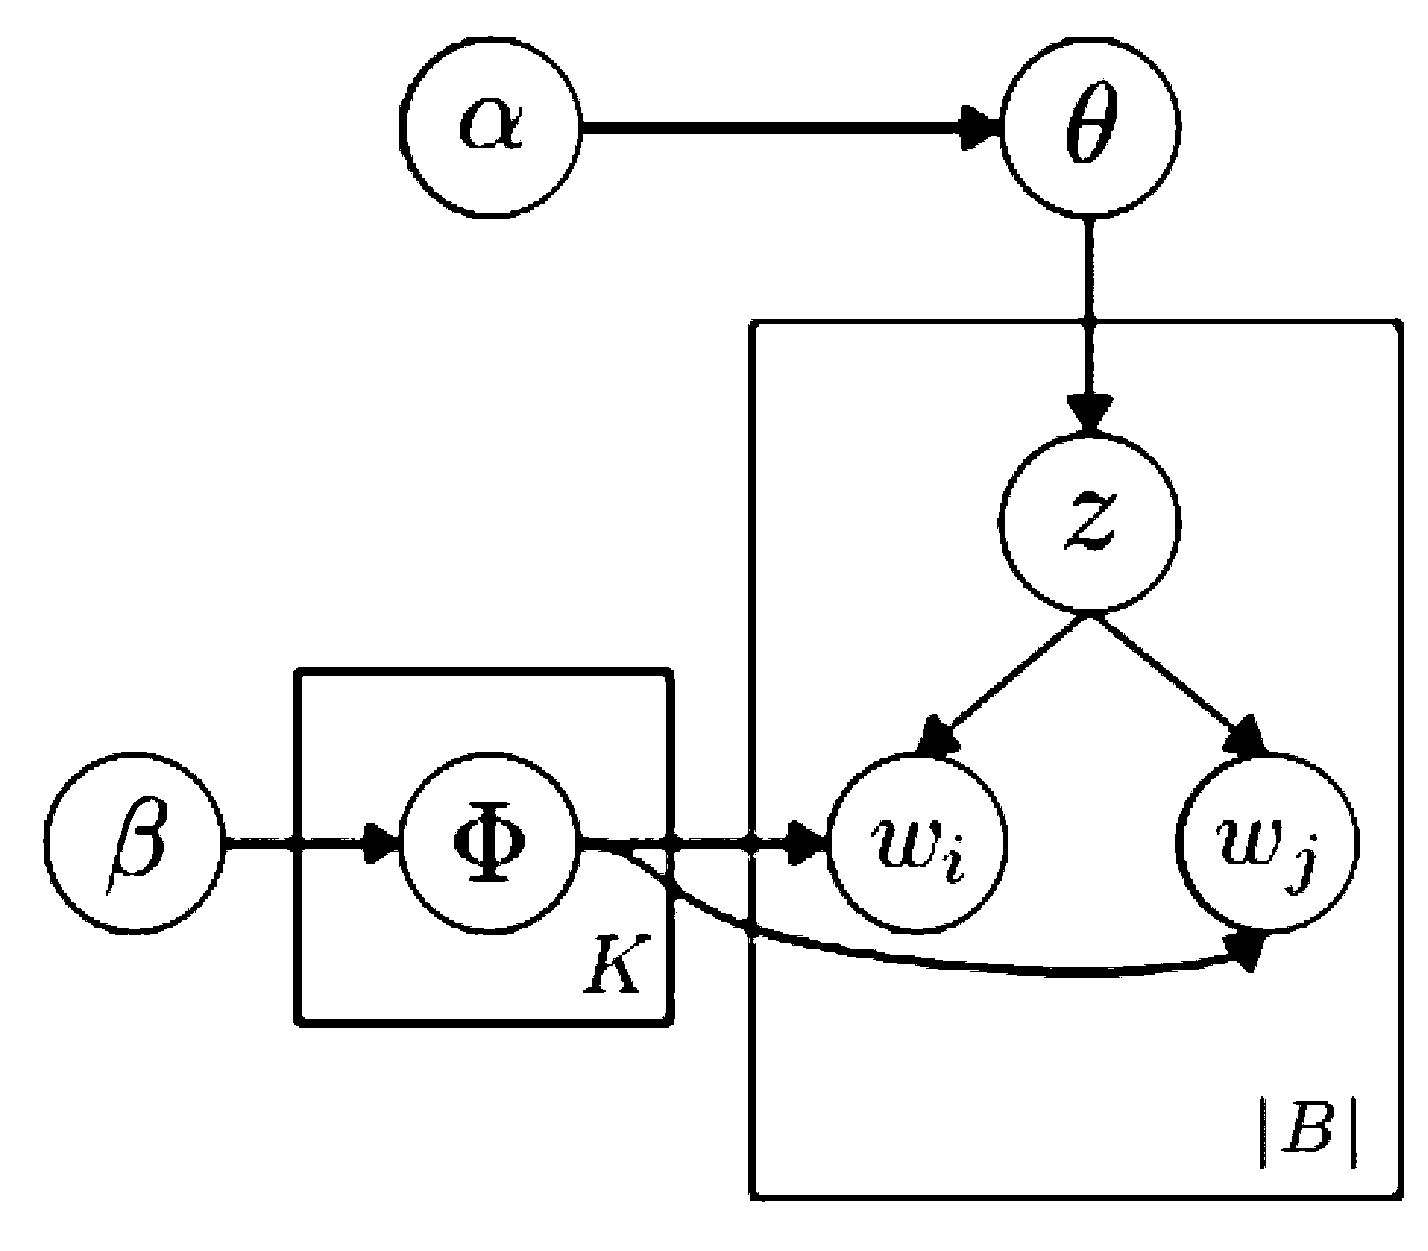
\includegraphics[scale=1.0]{graphicalBTM}
	}
	\caption{Graphical BTM plate representation.}\label{fig:graphicalBTM}
\end{figure}

In generating biterm from a document corpus, BTM directly removes stop word and then generate biterm based on the initialised fixed-size sliding window. This probability method drew of couple words or biterm to a specific topic. The steps of BTM generative process introduced in \cite{YanGuoLan,ChengYanLan} can be written as the following:
\begin{itemize}
	\item for each topic \(z\):
	\begin{enumerate}
		\item draw a topic-specific word distribution \(\Phi_z \sim \textit{Dir}(\beta)\);
	\end{enumerate}
	\item draw a topic proportion vector \(\theta \sim \textit{Dir}(\alpha)\) for the whole collection;
	\item  for each biterm \(b\) in set \(B\):
	\begin{enumerate}
		\item draw a topic assignment \(z \sim \textit{Multi}(\theta)\),
		\item draw two words: \(w_i, w_j \ sim \textit{Multi}(\Phi_z)\).
	\end{enumerate}
\end{itemize}

In BTM the initial number topic \(z\) contained the sum of topic-specific word distribution from the whole collection. It is indicating that for each biterm in set \(B\) is assign random topic as the initial state. The detail extraction word-pairs from corpus as the following equation \cite{XuLiuWu}:
\begin{equation}
	\label{eqn:17}
	\textit{GenBiterm}(\textit{words}) = \sum_{i=1}^{N-1} \sum_{j = 1}^{N}\textit{biterm}(w_i, w_j).
\end{equation}

In the process of extraction as in equation~\cref{eqn:17} is necessary to determine the size of sliding window, and the word-pairs is given a unique identifier to prevent duplicate with assumption generated word-pairs \(\textit{biterm}(w_i,w_j)\) is equal to \(\textit{biterm}(w_j,w_i)\). The output from this process is set \(\textit{biterm } B\), which directly model the word co-occurrences in the whole corpus to make full use of the global information \cite{WangZhangLiu}.

In the development of BTM, Yen et al., were using collapsed Gibbs Sampling \cite{Griffiths} to conjugate out priors, where have contained three latent variables \(z\), \(\Phi \), and \(\theta \). The latent variables can be integrated out using \(\alpha\) and \(\beta\). They were calculating \(P(z \vert z_{\neg b}, B, \alpha, \beta)\) for each \(z_{\neg b}\), where \(z_{\neg b}\) denotes the topic assignments for all biterms except \(b, B\) is the global biterm set. The joint probability of all the data was using conditional probability as the such equation \cite{YanGuoLan,HeXuLi}:
\begin{equation}
	\label{eqn:18}
	P(z \mid z_{\neg b}, B, \alpha, \beta) \varpropto (n_z + \alpha) \frac{(n_{w_i \vert z} + \beta)(n_{w_j \vert z} + \beta)}{(\sum_{w} n_{w_i \vert z} + M\beta)^2}
\end{equation}
where \(n_z\) is the number of times of the biterm \(b\) assigned to the topic \(z\), and \(n_{w \vert z}\) is the number of times of the word \(w\) assigned to the topic \(z\). In \cite{YanGuoLan,ChengYanLan} have determined that when the biterm has assigned to a topic, both of \(w_i\) and \(w_j\) actually assigned to the same topic.

For each biterm in set \(B\) iteration always calculate and update the biterm information by assigning to a specific topic using equation~\cref{eqn:18}. After period times of iteration has been performed, it will be easily estimated topic-word distribution \(\Phi\) and global-topic distribution \(\theta\) using the equations \cite{YanGuoLan}
\begin{equation}
	\label{eqn:19}
	\Phi_{w \vert z} = \frac{n_{w \vert z}  + \beta}{\sum_{w} n_{w \vert z} + M\beta}
\end{equation}
\begin{equation}
	\label{eqn:20}
	\theta_{z} = \frac{n_{z}  + \alpha}{\lvert B \rvert + K\alpha}.
\end{equation}

The output of topic-word distribution in equation~\cref{eqn:19} and global-topic distribution in equation~\cref{eqn:20} can be stored in a file or database in the table form, where the rows are all unique words in the entire documents collection or single row for global-topic; the columns are all topics of the collection.

BTM can infer a topic in a document by using the equation
\begin{equation}
	\label{eqn:21}
	P(z \vert d) = \sum_{b}P(z \vert d)P(b \vert d),
\end{equation} here the \(P(z \vert d)\) can be calculated by using Bayes formula as follows:

\begin{equation}
	\label{eqn:22}
	P(z \vert b) = \sum P(z \vert d) P(b \vert d) \frac{P(z) P(w_i \vert z) P(w_j \vert z)}{\sum_{z} P(z) P(w_i \vert z) P(w_j \vert z)}.
\end{equation}

In formula~\cref{eqn:22} \(P(z)\) is global topic proportion \(\theta_z\); \(P(w \vert z)\) is topic-word distribution \(\Phi_{i \vert z}\). To obtain probability \(P (b \vert d)\) as in equation~\cref{eqn:21}, the distribution of biterm in the document can be estimated by the following equation:
\begin{equation}
	\label{eqn:23}
	P (b \vert d) = \frac{n_d(b)}{\sum_{b} n_d(b)},
\end{equation} where \(n_d\) is the frequency of generated biterm \(b\) in document \(d\).

In order to evaluate topic quality, Mimno et al. \cite{MimnoWallachTalley}, proposed topic coherence measure that corresponds well with human coherence judgments and makes it possible to identify specific semantic problems in topic models without human evaluations or external reference corpora as follows:
\begin{equation}
	\label{eqn:24}
	C(t; V^{(t)}) = \sum_{m = 2}^{M} \sum_{l = 2}^{m - 1} \log{\frac{D(v_m^{(t)} v_l^{(t)}) + 1}{D(v_l^{(z)})}}
\end{equation}

In formula~\cref{eqn:24} \(D(v)\) is word document frequency type \(v\), \(D(v,v')\) is co-word document frequency type \(v\) and \(v'\). \(V^{(t)} = (v_1^{(t)} \dots v_M^{(t)})\) is the list top-\(M\) most probable word in each topic \(t\). Smoothing count value is one, in order to avoid zero number in logarithm calculation. This coherence measure is sometimes called UMass metric which is more intrinsic in nature, it attempts to confirm that the models learned data known to be in the corpus \cite{StevensKegelmeyerAndrzejewski}.

\paragraph{Proposed BTM input feature.} The fundamental idea of BTM is that if two words co-occur more frequently, they are more likely to belong to the same topic \cite{ChengYanLan} with the assumption that generated word-pair of documents will be drawn independent from the topic. Starting from that assumption, we incorporate TVM indices function to calculate TF-IDF weighting score to adjust a feature for each biterm in set \(B\).

As our concern on providing a list of document collections which thematically similar with given the word or document query, we pay attention on the third step of BTM generative process. This issue also has been revised in d-BTM \cite{XiaTangHussain} proposed by Xia et al., where they have focused on biterm discrimination \(w_i - w_j\). However, in our method, we prepare a biterm set \(B\), then assign biterm feature based on word-pairs \(w_i\) and \(w_j\). The weighting pair of \(w_i\) and \(w_j\) are using numerical statistic TF-IDF method \cite{ManningRaghavanSchutze,ZhangYoshidaTang} for measuring how important the word in the document, where term frequency is logarithm \((L)\), document frequency is inverse document frequency of term \((T)\) and normalisation is pivot unique \((U)\). The Logarithm-Term-Pivoted Unique \((LTU)\) combination of TF-IDF as follows:
\begin{equation}
	\label{eqn:25}
	\text{TF} = 1 + \log{(tf_{t, d})},
\end{equation}
\begin{equation}
	\label{eqn:26}
	\text{IDF} = \log{(1 + N / df_b)},
\end{equation}
\begin{equation}
	\label{eqn:27}
	\text{Norm} = 1 / N_t,
\end{equation}
\begin{equation}
	\label{eqn:28}
	\text{TD-IDF} = \text{TF}.\text{IDF}.\text{Norm},
\end{equation}
here \(tf_{t,d}\) is a number of times a term appeared in global generated document sliding window, \(N\) is the total number biterm in set \(B\), \(df_b\) is a number of times biterm co- occurrence in global generated document sliding window, \(N_t\) is the number of unique terms in set \(B\). By taking advantage feature of the term and biterm co-occurrence from document sliding window, we adopt TF-IDF model calculation to formulate weighting score that will be used as a BTM input feature.

\paragraph{Experiments and results.} The experiment carried out to evaluate input parameter feature in BTM that have been proposed using TF-IDF variance as in equations~\cref{eqn:25,eqn:26,eqn:27,eqn:28} and comparing the output with Standard BTM feature; we also perform topic labelling document cluster using our proposed feature parameter of BTM. In this experiment, we have used Intel Xeon Processor E5-2620 v4 (Broadwell) 2.1 GHz, memory DDR4 32 Gb, and hard disk Skyhawk Surveillance 2 Terabyte. The documents have used in this experiment based on thematic virtual museums (TVM) corpus that contained 29.362 collections \cite{AnggaiBlekanovSergeev2018}, that reduced to 23.485 in minimum two terms contained in a document.

In order to compare Standard BTM with our proposed input feature, we were performing difference \(K\)-topics number, inferring all words which were containing in \(K\)-topics, and applying standard intrinsic UMass method for measuring topic coherence. We count average coherence score of Top-\(N\) words for each \(K\)-topics \cite{YanGuoLan}, the higher score is indicating better performance. In all cases, we defined \(a = 50/K\), \(b = 0.01\), and Top-\(N = 10\). The calculation result based on UMass coherence measure as shown in Table~\cref{tab:umassCalculationResults}.

\begin{table} [htbp]%
	\centering
	\caption{Calculation result based on UMass coherence measure.}%
	\label{tab:umassCalculationResults}% label всегда желательно идти после caption
	\renewcommand{\arraystretch}{1.5}%% Увеличение расстояния между рядами, для улучшения восприятия.
	\begin{SingleSpace}
		\begin{tabulary}{\textwidth}{@{}>{\zz}L >{\zz}C >{\zz}C >{\zz}C >{\zz}C >{\zz}C  >{\zz}C@{}} %Вертикальные полосы не используются принципиально, как и лишние горизонтальные (допускается по ГОСТ 2.105 пункт 4.4.5) % @{} позволяет прижиматься к краям
			\toprule     %%% верхняя линейка
			Iteration & Method & \(K = 10\) & \(K = 20\) & \(K = 50\) & \(K = 70\) & \(K = 100\)\\
			\midrule %%% тонкий разделитель. Отделяет названия столбцов. Обязателен по ГОСТ 2.105 пункт 4.4.5
			100 & Feature BTM  & -33.77 & -38.74 & -53.42 & -52.96 & -53.57 \\
			& Standard BTM & -61.37 & -58.46 & -59.85 & -59.26 & -58.08 \\
			200 & Feature BTM & -35.56 &  -39.06 & -52.18 & -52.62 & -53.84 \\
			& Standard BTM & -61.93 & -59.56 & -52.18 & -58.56 & -58.53 \\
			300 & Feature BTM & -36.64 & -39.72 & -52.10 & -52.40 & -53.92 \\
			& Standard BTM & -60.66 & -57.70 & -59.87 & -58.34 & -59.35  \\
			400 & Feature BTM & -35.82 & -39.90 & -51.87 & -52.34 & -54.04 \\
			&  Standard BTM & -60.95 & -56.67 & -59.72 & -58.37 & -58.94  \\
			500 & Feature BTM & -35.97 & -40.09 & -51.71 & -52.06 & -54.17  \\
			& Standard BTM & -60.02 & -57.07 & -60.25 & -52.06 & -58.83 \\
			1000 & Feature BTM & -35.68 & -40.15 & -51.95 & -52.06 & -54.74 \\
			& Standard BTM &-60.97 & -58.25 & -60.22 & -60.22 & -60.22 \\
			\bottomrule %%% нижняя линейка
		\end{tabulary}%
	\end{SingleSpace}
\end{table}

Table~\cref{tab:umassCalculationResults} shows the approximately average scores for each \(K\)-dimensional topic and number iterations of Standard BTM and Feature BTM, where the calculation of coherence score have performed each ten times iteration in order to get a more precise average score. One can be noticed that our proposed method gives significant improvement of topic quality with a \(t\)-test on \(p\)-value less than 0.001. The detail graphic visualisation of Table calculation result based on UMass coherence measure as shown in Fig.~\cref{fig:umassCalculationResults}.

\begin{figure}[ht]
	\centerfloat{
		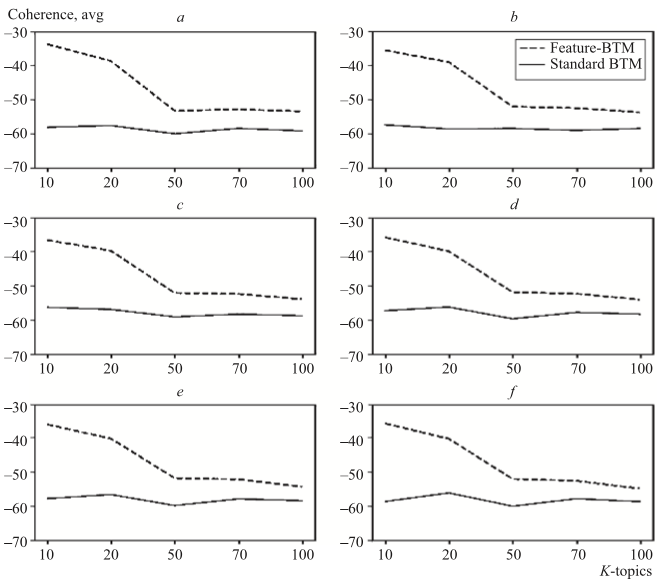
\includegraphics[scale=0.6]{umassCalculationResults}
	}
	\legend{Iterations: \(a\) -- 100, \(b\) -- 200, \(c\) -- 300, \(d\) -- 400, \(e\) -- 500, \(f\) -- 1000.}
	\caption{Calculation result based on UMass coherence measure.}\label{fig:umassCalculationResults}
\end{figure}

In Fig.~\cref{fig:umassCalculationResults}, the average coherence score presented for each \(K\)-dimensional topics in the single graph can be more clearly investigated, where the average gap coherence score between Standard BTM and our proposed method were small when the K-dimensional increased. This explained by the fact that at \(K\) number from 10 to 50, the method well identifies and underestimates the weight of biterms frequently used, which in the case of Standard BTM with such \(K\) fall into almost all topics.

In viewing topic model as a method for dimensional reduction, we performed experiments to cluster the documents based on the TVM corpus and assign to a specific cluster label. The process of assigned a topic cluster to a document as follows. The first step, for each topic \(j (j \in K)\) infer \(N\) documents and for each document \(N_i\) the total probability of the all words occurrence of this document in each topic (or the overall relevance of the document to the topic) was calculated -- \(P_{ij}\). Second, we choose the highest probability score for each document max \(f\) \((P_{ij})\). Finally, each cluster \(j\) assigned only to those 

In this experiment, we define number of topic \(K = 100\) with 1000 iterations for per- forming dimensional reduction by clustering TVM corpus based on a modification of BTM input feature, the cluster results based on UMass coherence measure as shown in Fig.~\cref{fig:umassClusterResults}.
documents that have the highest relevance value.

\begin{figure}[ht]
	\centerfloat{
		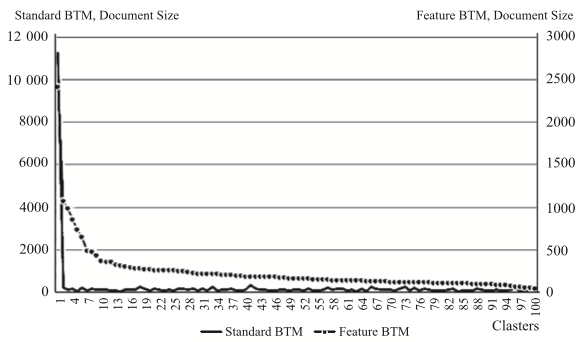
\includegraphics[scale=0.6]{umassClusterResults}
	}
	\caption{Cluster results based on UMass coherence measure.}\label{fig:umassClusterResults}
\end{figure}

Time for calculating input parameter weighting score was exemplarily 0.002 seconds, the total time for each update iteration was exemplarily 27.26 minutes, and the average was exemplarily 0.027 minutes, calculating and normalising \(\Phi\) and \(\theta\) was exemplarily 9.25 seconds, while total time for inferring document collections and assigning topic label was exemplarily 17.29 seconds. Based on these calculation, we can estimate the total time needed for calculating proposed input feature of BTM is approximately 27.75 minutes. As shown in Fig.~\cref{fig:umassClusterResults}, minimum cluster size of the TVM corpus after the Standard BTM applied was 34, maximum class size was 11.275 documents, while our proposed BTM input feature, the minimum cluster size was 39 with maximal class size was 2.421 documents. We found that our proposed method gives better number document proportion of clusters than the Standard BTM. By performing topic cluster, we have reduced query time operation for retrieving relevant information in the whole documents to local documents in a cluster which related to a given query document.

\paragraph{Conclusion.} In this paper we have proposed to exploit BTM input feature parameter based on the modification of the third step of the generative process. Experimental results shown the advantage of efficiency by the modified Feature BTM model before the Standard BTM model. The thematic clustering technology of documents necessary for creation of thematic virtual museums has described. The authors performed a performance evaluation, that shown a slight loss of speed (less than 30 seconds), more effective used the Feature BTM for clustering the virtual museum collection than the Standard BTM model.

\section{Оптимальное конструирование сборщика (цепочка роботов)}\label{sec:ch4/sect3}

\section{Реализация программного комплекса}\label{sec:ch4/sect4}

\FloatBarrier

